\documentclass[article]{jss}
% \usepackage{draftwatermark}
% \SetWatermarkText{Draft}
% \SetWatermarkScale{2}
\newif\ifen
\newif\ifes
\newcommand{\en}[1]{\ifen#1\fi}
\newcommand{\es}[1]{\ifes#1\fi}
\entrue
\usepackage[utf8]{inputenc}

%\newcommand{\jan}{%
%  \en{January}%
%  \es{Enero}
%}

\usepackage{caption}
\usepackage{subcaption}
\usepackage{amsmath} %para escribir funci\'on partida , matrices
\usepackage{amsthm} %para numerar definciones y teoremas
\usepackage{amsfonts} % \mathbb{N} -> conjunto de los n\'umeros naturales

\usepackage{bm} % \bm{\alpha} bold greek symbol
\usepackage[makeroom]{cancel} % \cancel{} \bcancel{} etc
\usepackage{wrapfig} % \begin{wrapfigure} Pone figura al lado del texto
\usepackage{mdframed}
\usepackage{algorithm}
\usepackage{comment}
%\usepackage{quoting}
\usepackage{mathtools}
\usepackage{tikz}
\usepackage{csvsimple}
\usepackage{listings}
\usepackage{hyperref}
\usepackage{todonotes}
\definecolor{dkgreen}{rgb}{0,0.6,0}
\definecolor{mauve}{rgb}{0.58,0,0.82}


% tikzlibrary.code.tex
%
% Copyright 2010-2011 by Laura Dietz
% Copyright 2012 by Jaakko Luttinen
%
% This file may be distributed and/or modified
%
% 1. under the LaTeX Project Public License and/or
% 2. under the GNU General Public License.
%
% See the files LICENSE_LPPL and LICENSE_GPL for more details.

% Load other libraries

%\newcommand{\vast}{\bBigg@{2.5}}
% newcommand{\Vast}{\bBigg@{14.5}}
% \usepackage{helvet}
% \renewcommand{\familydefault}{\sfdefault}

\usetikzlibrary{shapes}
\usetikzlibrary{fit}
\usetikzlibrary{chains}
\usetikzlibrary{arrows}

% Latent node
\tikzstyle{latent} = [circle,fill=white,draw=black,inner sep=1pt,
minimum size=20pt, font=\fontsize{10}{10}\selectfont, node distance=1]
% Observed node
\tikzstyle{obs} = [latent,fill=gray!25]
% Invisible node
\tikzstyle{invisible} = [latent,minimum size=0pt,color=white, opacity=0, node distance=0]
% Constant node
\tikzstyle{const} = [rectangle, inner sep=0pt, node distance=0.1]
%state
\tikzstyle{estado} = [latent,minimum size=8pt,node distance=0.4]
%action
\tikzstyle{accion} =[latent,circle,minimum size=5pt,fill=black,node distance=0.4]
\tikzstyle{fijo} =[latent,circle,minimum size=5pt,fill=black]


% Factor node
\tikzstyle{factor} = [rectangle, fill=black,minimum size=10pt, draw=black, inner
sep=0pt, node distance=1]
% Deterministic node
\tikzstyle{det} = [latent, rectangle]

% Plate node
\tikzstyle{plate} = [draw, rectangle, rounded corners, fit=#1]
% Invisible wrapper node
\tikzstyle{wrap} = [inner sep=0pt, fit=#1]
% Gate
\tikzstyle{gate} = [draw, rectangle, dashed, fit=#1]

% Caption node
\tikzstyle{caption} = [font=\footnotesize, node distance=0] %
\tikzstyle{plate caption} = [caption, node distance=0, inner sep=0pt,
below left=5pt and 0pt of #1.south east] %
\tikzstyle{factor caption} = [caption] %
\tikzstyle{every label} += [caption] %

\tikzset{>={triangle 45}}

%\pgfdeclarelayer{b}
%\pgfdeclarelayer{f}
%\pgfsetlayers{b,main,f}

% \factoredge [options] {inputs} {factors} {outputs}
\newcommand{\factoredge}[4][]{ %
  % Connect all nodes #2 to all nodes #4 via all factors #3.
  \foreach \f in {#3} { %
    \foreach \x in {#2} { %
      \path (\x) edge[-,#1] (\f) ; %
      %\draw[-,#1] (\x) edge[-] (\f) ; %
    } ;
    \foreach \y in {#4} { %
      \path (\f) edge[->,#1] (\y) ; %
      %\draw[->,#1] (\f) -- (\y) ; %
    } ;
  } ;
}

% \edge [options] {inputs} {outputs}
\newcommand{\edge}[3][]{ %
  % Connect all nodes #2 to all nodes #3.
  \foreach \x in {#2} { %
    \foreach \y in {#3} { %
      \path (\x) edge [->,#1] (\y) ;%
      %\draw[->,#1] (\x) -- (\y) ;%
    } ;
  } ;
}

% \factor [options] {name} {caption} {inputs} {outputs}
\newcommand{\factor}[5][]{ %
  % Draw the factor node. Use alias to allow empty names.
  \node[factor, label={[name=#2-caption]#3}, name=#2, #1,
  alias=#2-alias] {} ; %
  % Connect all inputs to outputs via this factor
  \factoredge {#4} {#2-alias} {#5} ; %
}

% \plate [options] {name} {fitlist} {caption}
\newcommand{\plate}[4][]{ %
  \node[wrap=#3] (#2-wrap) {}; %
  \node[plate caption=#2-wrap] (#2-caption) {#4}; %
  \node[plate=(#2-wrap)(#2-caption), #1] (#2) {}; %
}

% \gate [options] {name} {fitlist} {inputs}
\newcommand{\gate}[4][]{ %
  \node[gate=#3, name=#2, #1, alias=#2-alias] {}; %
  \foreach \x in {#4} { %
    \draw [-*,thick] (\x) -- (#2-alias); %
  } ;%
}

% \vgate {name} {fitlist-left} {caption-left} {fitlist-right}
% {caption-right} {inputs}
\newcommand{\vgate}[6]{ %
  % Wrap the left and right parts
  \node[wrap=#2] (#1-left) {}; %
  \node[wrap=#4] (#1-right) {}; %
  % Draw the gate
  \node[gate=(#1-left)(#1-right)] (#1) {}; %
  % Add captions
  \node[caption, below left=of #1.north ] (#1-left-caption)
  {#3}; %
  \node[caption, below right=of #1.north ] (#1-right-caption)
  {#5}; %
  % Draw middle separation
  \draw [-, dashed] (#1.north) -- (#1.south); %
  % Draw inputs
  \foreach \x in {#6} { %
    \draw [-*,thick] (\x) -- (#1); %
  } ;%
}

% \hgate {name} {fitlist-top} {caption-top} {fitlist-bottom}
% {caption-bottom} {inputs}
\newcommand{\hgate}[6]{ %
  % Wrap the left and right parts
  \node[wrap=#2] (#1-top) {}; %
  \node[wrap=#4] (#1-bottom) {}; %
  % Draw the gate
  \node[gate=(#1-top)(#1-bottom)] (#1) {}; %
  % Add captions
  \node[caption, above right=of #1.west ] (#1-top-caption)
  {#3}; %
  \node[caption, below right=of #1.west ] (#1-bottom-caption)
  {#5}; %
  % Draw middle separation
  \draw [-, dashed] (#1.west) -- (#1.east); %
  % Draw inputs
  \foreach \x in {#6} { %
    \draw [-*,thick] (\x) -- (#1); %
  } ;%
}



\newcommand{\vm}[1]{\mathbf{#1}}
\newcommand{\N}{\mathcal{N}}
\newcommand\hfrac[2]{\genfrac{}{}{0pt}{}{#1}{#2}} %\frac{}{} sin la linea del medio

\usepackage{listings}
\lstset{
  language=Python,
  aboveskip=3mm,
  belowskip=3mm,
  showstringspaces=true,
  columns=flexible,
  basicstyle={\small\ttfamily},
  numbers=none,
  numberstyle=\tiny\color{gray},
  keywordstyle=\color{blue},
  commentstyle=\color{dkgreen},
  stringstyle=\color{mauve},
  breaklines=true,
  breakatwhitespace=true,
  tabsize=4
}


%% -- LaTeX packages and custom commands ---------------------------------------

%% recommended packages
\usepackage{thumbpdf,lmodern}

%% another package (only for this demo article)
\usepackage{framed}

%% new custom commands
\newcommand{\class}[1]{`\code{#1}'}
\newcommand{\fct}[1]{\code{#1()}}

 
%% -- Article metainformation (author, title, ...) -----------------------------

%% - \author{} with primary affiliation
%% - \Plainauthor{} without affiliations
%% - Separate authors by \And or \AND (in \author) or by comma (in \Plainauthor).
%% - \AND starts a new line, \And does not.
\author{Gustavo Landfried \\Universidad de Buenos Aires
   \And Matias Mazzanti \\Universidad de Buenos Aires
   \And Esteban Mocskos \\Universidad de Buenos Aires}
\Plainauthor{Gustavo Landfried, Matias Mazzanti, Esteban Mocskos }

%% - \title{} in title case
%% - \Plaintitle{} without LaTeX markup (if any)
%% - \Shorttitle{} with LaTeX markup (if any), used as running title
\title{All the concepts behind TrueSkill Through Time: the \proglang{R}, \proglang{Python} and \proglang{Julia} packages (Draft)}
\Plaintitle{All the concepts behind TrueSkill Through Time: the R, Python and Julia packages (Draft)}
\Shorttitle{TrueSkill Through Time: the \proglang{R}, \proglang{Python} and \proglang{Julia} packages (Draft)}

%% - \Address{} of at least one author
%% - May contain multiple affiliations for each author
%%   (in extra lines, separated by \emph{and}\\).
%% - May contain multiple authors for the same affiliation
%%   (in the same first line, separated by comma).
\Address{
  Gustavo Andr\'es Landfried\\
  Departamento de Computaci\'on\\
  Facultad de Ciencias Exactas y Naturales\\
  Universidad de Buenos Aires\\
  Buenos Aires, Argentina\\
  E-mail: \texttt{gustavolandfried@gmail.com}\\

  \vspace{0.3cm}

  Matias Mazzanti\\
  Departamento de F\'isica\\
  Facultad de Ciencias Exactas y Naturales\\
  Universidad de Buenos Aires\\
  Buenos Aires, Argentina\\

  \vspace{0.3cm}

  Esteban Mocskos\\
  Departamento de Computaci\'on\\
  Facultad de Ciencias Exactas y Naturales\\
  Universidad de Buenos Aires\\
  Buenos Aires, Argentina\\
  \emph{and}\\
  Departamento de Computaci\'on\\
  Facultad de Ciencias Exactas y Naturales\\
  Universidad de Buenos Aires\\
  Buenos Aires, Argentina\\
}




























%% - \Abstract{} almost as usual
\Abstract{
 \en{Humans develop complex skills through time.}
 \es{Los humanos desarrollan habilidades complejas a través del tiempo.}
 %
 \en{Knowing how they change is crucial in many areas, such as educational systems and the video game industry.}
 \es{Saber c\'omo cambian es crucial en muchas \'areas, como los sistemas educativos y la industria de los videojuegos.}
 %
 \en{All widely used skill estimators share the same underlying causal model, but differ in their inferential procedure.}
 \es{Todos los estimadores de habilidad ampliamente utilizados comparten el mismo modelo causal subyacente, pero se diferencian en sus procedimientos metodol\'ogicas.}
 %
 \en{The success of TrueSkill was based on the application of an efficient algorithm to find the best approximation of the exact posterior.}
 \es{El éxito del TrueSkill se bas\'o en la aplicaci\'on de un algoritmo eficiente para encuentrar la mejor aproximaci\'on del posterior exacto.}
 %
 \en{TrueSkill Through Time is a major enhancement that uses a single generative model for the entire history of activities, rather than a sequence of independent observations, allowing historical information to propagate throughout the system, resulting in better estimates with even less data.}
 \es{TrueSkill Through Time utiliza un único modelo generativo para toda la historia de las actividades, en lugar de una secuencia de observaciones independientes, lo que permite que la informaci\'on hist\'orica se propague por todo el sistema, lo que da lugar a mejores estimaciones con aún menos datos.}
 %
 \en{The use of an efficient algorithm, that requires only a few linear iterations over the data, allows scaling to millions of observations in few minutes.}
 \es{El uso de un algoritmo eficiente, que requiere s\'olo unas pocas iteraciones lineales sobre los datos, permite escalar a millones de observaciones en pocos minutos.}
 %
 \en{This paper offer the first packages for \proglang{R}, \proglang{Python} and \proglang{Julia}, together with its scientific documentation.}
 \es{Mediante este art\'iculo ofrecemos los primeros paquetes para \proglang{R}, \proglang{Python} y \proglang{Julia}, junto con su documentaci\'on cient\'ifica.}
}
\Keywords{Life history, skill, learning, education, sports, gaming, inference, \proglang{R}, \proglang{Python}, \proglang{Julia}}
\Plainkeywords{}


% Para fijar que la siguiente cita la incluya como primer autor y et al. Usar con citas de muchos autores.
\shortcites{Koster2020}


\begin{document}
\lstset{language=Python}

\section[Introduction]{Introduction: } \label{sec:intro}

\en{Humans acquire and develop complex skills over the course of a lifetime.}
\es{Los humanos desarrollan habilidades complejas a lo largo de su vida.}
%
\en{This is possible by a combination of different biological, cognitive and social processes~\citep{Koster2020}.}
\es{Esto es posible gracias a una integraci\'on especial de los procesos biol\'ogicos, cognitivos y sociales~\citep{Koster2020}.}
%
\en{Our specie is characterized by first developing the brain and then the body to allow a longer period of learning~\citep{GonzalezForero2018}.}
\es{Nuestros cerebros se desarrollan primero, seguidos por el cuerpo porque esta secuencia permite un per\'iodo m\'as largo de aprendizaje~\citep{GonzalezForero2018}.}
%
% \en{Human life histories are distinguished by long periods of juvenile dependency, short intervals between births, and long postreproductive life span~\citep{Jones2011}.}
% \es{Las historias de vida humanas se distinguen por largos per\'iodos de dependencia juvenil, cortos intervalos entre nacimientos y una larga vida posreproductiva~\citep{Jones2011}.}
%
\en{A special cognitive ability allows humans to learn things from others, and transmit innovations through generations~\citep{Herrmann2007}.}
\es{Una capacidad cognitiva especial le permite a los humanos aprender de los dem\'as y transmitir las innovaci\'on a través de la generaciones~\citep{Herrmann2007}.}
%
\en{As a population-based process, human adaptation is also affected by demographic characteristics, such as the size and structure of populations~\citep{derex2020-populationStructure}.}
\es{Al ser un proceso poblacional, la adaptaci\'on humana también se ve afectada por caracter\'isticas demogr\'aficas, como el tama\~no y estructura de las poblaciones~\citep{derex2020-populationStructure}.} 

% Parrafo

\en{Understanding the factors impacting in the positive or negative changes of skill could be used to develop new training strategies or adapting the environment to avoid unnecessary tasks.}
\es{Conocer c\'omo cambian la habilidades de la personas en el tiempo es crucial en muchas \'areas.}
%
\en{For example, in sports development and education, knowing the skill and how it changes can serve to avoid exposing agents to imbalanced challenges, maintain the interest and engagement.}
\es{En contextos educativos, calificaciones precisas pueden servir para evitar exponer a los agentes a desaf\'ios desproporcionados, estimulando as\'i el inter\'es y la participaci\'on.}
%
\en{For research purposes, they can help to refine and test models of human learning.}
\es{Con fines de investigaci\'on, ellas pueden ayudar a refinar y testear modelos de aprendizaje humano.}
%
\en{In practice, since skill is a hidden variable, the best we can do is estimate it from its direct observable consequences.}
\es{En la pr\'actica, dado que la habilidad es una variables oculta, lo mejor que podemos hacer es estimarla a partir de sus consecuencias observables m\'as directas.}
%
\en{The most widely used sources of information in education and sports are the outcomes of problem solving and competition between opponents.}
\es{Las fuentes de informaci\'on m\'as utilizadas en educaci\'on y deportes provienen del producto de resoluci\'on de problemas y de competencia entre oponentes.}
%
\en{The naive solution, frequency of positive results, is not a good indicator essentially because it also depends on the difficulty of the challenges.}
\es{La soluci\'on ingenua, frecuencia de resultados positivos, no es un buen indicador fundamentalmente porque depende tambi\'en de la dificultad de los desaf\'ios.}
%
\en{For that reason, all solutions rely on pairwise comparisons.}
\es{Por esa raz\'on, todos las soluciones se basan en comparaciones entre pares.}
%
\en{Since the first generative models, proposed almost a century ago by~\cite{thurstone1927-comparativeJugement} and~\cite{zermelo1929-translation}, it is assumed that the probability of an observed result, $r_{ij}$, depends on the difference in performance, $d_{ij}$, between the agent $i$ and target $j$, $P(\, r_{ij} \,|\, d_{ij} \,)$.}
\es{Ya los primeros modelos generativos, propuestos hace casi un siglo por~\cite{thurstone1927-comparativeJugement} y~\cite{zermelo1929-translation}, suponen que la probabilidad de un resultado observado, $r$, depende de la diferencia de rendimiento, $d$, entre el agente y su objetivo, $P(\, r_{ij} \,|\, d_{ij} \,)$.}
%
\en{The field revitalized 20 years later by the publications of~\cite{bradley1952-pairedComparisions} and~\cite{mosteller1951-remarks}.}
\es{El campo revitaliz\'o 20 a\~nos despu\'es gracias a las publicaciones de \cite{bradley1952-pairedComparisions} y~\cite{mosteller1951-remarks}.}

\todo[inline]{Hay que decir porque es importante la publicacion de Bradley y Mosteller} 
% Parrafo

\en{Nowadays, the most widely used skill estimators were proposed by~\cite{elo1961-uscf},~\cite{Glickman1999},~\cite{herbrich2006-trueskill}, and some of the Item-Response Theory variants compiled by~\cite{vanDerLinden2016-handbookIRT_1} and~\cite{fox2010-bayesianIRT}.}
\es{Actualmente, los estimadores de habilidades m\'as utilizados son los propuestos por~\cite{elo1961-uscf},~\cite{glikman_gliko_2},~\cite{herbrich2006-trueskill}, y algunas de las variantes de la\emph{Item-Response Theory} recopiladas por~\cite{vanDerLinden2016-handbookIRT_1} y~\cite{fox2010-bayesianIRT}.}
%
\en{Although they sometimes choose alternative bell-shape distributions to define the cumulative probability $P(\, d_{ij} > 0 \,)$, the underlying generative model is the same.}
\es{Por m\'as que a veces se usen distintas distribuciones \emph{bell-shape} para definir la probabilidad acumulada $P(\, d_{ij} > 0 \,)$, el modelo generativo subyacente es el mismo.}
%
\en{The main difference between them are methodological: the procedure to solve the shared probabilistic model.}
\es{Las principales diferencias ente ellos son metodol\'ogicas: el procedimiento para resolver el modelo probabil\'istico compartido.}
% Cambio de parrafo.
\begin{figure}[h!]
\centering \small
    \tikz{         
    \node[det, fill=black!10] (r) {$r_{ij}$} ; 
    \node[const, left=of r, xshift=-1.35cm] (r_name) {\small \en{Result}\es{Resultado}:}; 
    \node[const, right=of r] (dr) {\normalsize $ r_{ij} = (d_{ij}>0)$}; 

    \node[latent, above=of r, yshift=-0.45cm] (d) {$d_{ij}$} ; %
    \node[const, right=of d] (dd) {\normalsize $ d_{ij}=p_i-p_j$}; 
    \node[const, left=of d, xshift=-1.35cm] (d_name) {\small \en{Difference}\es{Diferencia}:};
    
    \node[latent, above=of d, xshift=-0.8cm, yshift=-0.45cm] (p1) {$p_i$} ; %
    \node[latent, above=of d, xshift=0.8cm, yshift=-0.45cm] (p2) {$p_j$} ; %
    \node[const, left=of p1, xshift=-0.55cm] (p_name) {\small \en{Performance}\es{Rendimiento}:}; 

    \node[accion, above=of p1,yshift=0.3cm] (s1) {} ; %
    \node[const, right=of s1] (ds1) {$s_i$};
    \node[accion, above=of p2,yshift=0.3cm] (s2) {} ; %
    \node[const, right=of s2] (ds2) {$s_j$};
    
    \node[const, right=of p2] (dp2) {\normalsize $p \sim \N(s,\beta^2)$};

    \node[const, left=of s1, xshift=-.85cm] (s_name) {\small \en{Skill}\es{Habilidad}:}; 
    
    \edge {d} {r};
    \edge {p1,p2} {d};
    \edge {s1} {p1};
    \edge {s2} {p2};
    %\node[invisible, right=of p2, xshift=4.35cm] (s-dist) {};
}
     \caption{
     \en{Generative model in which skills cause the observable results mediated by the difference of hidden performances.}
    \es{Modelo generativo en el que las habilidades causan los resultados observables a trav\'es de la diferencia de rendimientos ocultos.}
    %
    \en{At each event, agents exhibit a random performance around their true skill, $p \sim \N(s,\beta^2)$.}
    \es{En cada evento, los agentes exhiben una rendimiento aleatorio centrado en su verdadera habilidad, $p \sim \N(s,\beta^2)$.}
    %
    \en{The one with the highest performance wins, $r_{ij} = p_i > p_j$.}
    \es{Gana quien haya obtenido mayor rendimiento, $r_{ij} = p_i > p_j$.}
    %
    \en{The graphical representation defines a joint probability distribution.}
    \es{La representaci\'on gr\'afica define una distribuci\'on de probabilidad conjunta.}
    %
    \en{Observable variables are painted gray, hidden in white, and constants are shown as black dots.}
    \es{Las variables observables se pintan de gris, la ocultas en blanco, y las constantes se muestran como puntos negros.}
    %
    \en{The functions define the causal relationships.}
    \es{Las funciones definen las relaciones causales.}
    }
    \label{fig:generative_model}
\label{modelo}
\end{figure}
%
\en{A breakthrough took place with the methodology developed by~\cite{elo1961-uscf} for the US Chess Federation (USCF), which is still used by the International Chess Federation (FIDE).}
\es{Un gran avance produjo la metodolog\'ia desarrollada por~\cite{elo1961-uscf} para la Federaci\'on de Ajedrez de los Estados Unidos (USCF), adoptada hasta el d\'ia de hoy por la Federaci\'on Internacional De Ajedrez (FIDE).}
%
\en{Figure~\ref{fig:generative_model} provides a graphical representation in which skill generate observable results.}
\es{La figura~\ref{fig:generative_model} ofrece una representaci\'on gr\'afica en la que las habilidades generan los resultados observables.}
%
% \en{The causal relationship is not direct.}
% \es{La relaci\'on causal no es directa.}
% %
\en{However, the performance depends on an undetermined number of unknown factors, which are modeled with a constant noise, $\N(p\,|\,s,\beta^2)$.}
\es{El desempe\~no depende de una cantidad indeterminada de factores desconocidos, que se modelan con un ruido constante, $\N(p\,|\,s,\beta^2)$.}
%
\en{Then, the observed result is a direct consequence of the difference of those hidden performances, $d_{ij}=p_i - p_j$.}
\es{Luego, el resultado observado es consecuencias directa de la diferencia de esos rendimientos ocultos, $d_{ij}=p_i - p_j$.}
%
\en{The one with the highest performance wins, $r_{ij} = (d_{ij} > 0)$.}
\es{Gana quien haya obtenido mayor rendimiento, $r_{ij} = (d_{ij} > 0)$.}
%
\en{By observing a result we can deduce, given the hypotheses, the order of the hidden performances that actually occurred in that event, and its a priori probability.}
\es{Al observar un resultado podemos deducir, dadas las hip\'otesis, el orden de los rendimientos ocultos que en efecto ocurri\'o en ese evento, y su probabilidad a priori.}
%
\en{Elo's methodological solution is extremely simple and astute: update the current estimate based on our surprise.}
\es{La soluci\'on metodol\'ogica de Elo es extremadamente sencilla y astuta: actualizar la estimaci\'on actual en funci\'on de nuestra sorpresa.}
%
\begin{equation}
 \Delta_i = \underbrace{y_{ij}}_{\hfrac{\text{Direction}}{\text{(Sign)}}}\underbrace{\left(1-P(\,r_{ij}\,|\,s_i,s_j\,)\right)}_{\hfrac{\text{Magnitud}}{\text{(Surprise)}}}
\end{equation}
%
\en{Where $y_{ij}$ is $1$ for winners and $-1$ for losers, and the probability of the observed result given the a priori estimates can be derived from Figure~\ref{fig:generative_model} (details at section~\ref{sec:analyticalSolution}).}
\es{Donde $y_{ij}$ es $1$ para ganadores y $-1$ para perdedores y la probabilidad del resultado observado dadas las estimaciones a priori se puede derivar de la figura~\ref{fig:generative_model} (detalles en la secci\'on~\ref{sec:analyticalSolution}).}
%
\en{Unlikely results would indicate that the current estimates are not entirely correct and should be updated to a greater extent than if they had occurred as expected.}
\es{Los resultados poco probables indicar\'ian que las estimaciones actuales no son del todo correctas y deber\'ian actualizarse en mayor medida que si hubieran ocurrido como se esperaba.}
%
\begin{equation}\label{eq:elo_update}
 s_i^{\text{new}} = s_i^{\text{old}} + \Delta_i
\end{equation}
%
\en{This solution can recover the relative scale of the agents, starting from arbitrary initial values.}
\es{Esta soluci\'on puede recuperar la escala relativa de los agentes, partiendo de de valores iniciales arbitrarios.}
%
\en{However, it does have some major weaknesses.}
\es{Sin embargo, tiene algunas debilidades importantes.}
%
\en{Because of the lack of a notion of uncertainty about the estimates, what one agent loses in equation~\ref{eq:elo_update} is acquired by the other.}
\es{Debido a la falta de una noci\'on de incertidumbre sobre las estimaciones, lo que un agente pierde en la ecuaci\'on~\ref{eq:elo_update} lo adquiere el otro.}
%
\en{As newly estimates tend to generate high surprise, their presence can abruptly modify estimates that had already converged correctly.}
\es{Como las estimaci\'on nuevas tienden a generan alta sorpresa, su presencia puede modificar bruscamente estimaciones que ya hab\'ian convergido correctamente.}
%
\en{to break the symmetry of equation~\ref{eq:elo_update}, nn ad-hoc solution was proposed: reduce the impact of $\Delta$ based on how many times the agent was already seen by the system.}
\es{Para romper la simetr\'ia de la ecuaci\'on~\ref{eq:elo_update}, una soluci\'on ad-hoc fue propuesta: reducir el impacto de $\Delta$ en funci\'on de las veces que el agente ya fue visto por el sistema.}
%
\en{That is the role played by the K-factor used by the FIDE,  $s_i^{\text{new}} = s_i^{\text{old}} + \Delta_i K_i$.}
\es{Ese es rol que desempe\~na el K-factor usado por la FIDE, $s_i^{\text{new}} = s_i^{\text{old}} + \Delta_i K_i$.}

% Cambio de parrafo

% \en{Probability Theory provides us with a consistent framework for quantifying the uncertainty of our beliefs~\cite{bishop2006-PRML}.}
% \es{La Teor\'ia de la Probabilidad nos proporciona un marco consistente para cuantificar la incertidumbre de nuestras creencias~\citep{bishop2006-PRML}.}
% %
\en{The use of Probability Theory to handle uncertainty, known as Bayesian inference, was widely adopted because it has proven to be a extremely useful tool in practice.}
\es{El uso de la Teor\'ia de la Probabilidad para manejar la incertidumbre, conocida como inferencia bayesiana, se adopt\'o ampliamente porque ha demostrado ser una herramienta extremadamente útil en la pr\'actica.}
%
\en{But this is also a principled choice.}
\es{Esto no es una elecci\'on ad-hoc.}
%
\en{Any system that represent degrees of belief by a numerical value, consistent with classical deductive logic and a set of axioms encoding commonsense reasoning, will necessarily be isomorphic to Probability Theory~\citep{Cox1946,vanHorn2003-guideCoxTheorem}.}
\es{Cualquier sistema que represente grados de creencia mediante un valor num\'erico, consistente con la l\'ogica deductiva cl\'asica y un conjunto de axiomas que codifican el razonamiento de sentido común,  ser\'a necesariamente isom\'orfico a la Teor\'ia de la Probabilidad~\citep{Cox1946,vanHorn2003-guideCoxTheorem}.}
%
\en{All of the probabilistic inference, no matter how complex, can be solved in terms of two simple equations: the~\ref{eq:sum_rule} and the~\ref{eq:product_rule}.}
\es{Toda inferencia probabil\'istica, no importa cuan compleja ella sea, puede ser resuelta a trav\'es de dos simples ecuaciones: la~\ref{eq:sum_rule} y la~\ref{eq:product_rule}.}

\begin{equation} \label{eq:sum_rule}
 \tag{\en{sum rule}\es{regla de la suma}}
 P(x) = \sum_{y} P(x,y) \ \ \ \ \ \text{or} \ \ \ \ \ p(x) = \int p(x,y) \, dy
\end{equation}
%
\en{This means that any marginal distribution can be obtained by integrating or summing up the joint distribution over $y$.}
\es{Esto significa que cualquier distribuci\'on marginal se puede obtener integrando o sumando la distribuci\'on conjunta sobre $y$.}
%
\begin{equation}\label{eq:product_rule}
\tag{\en{product rule}\es{regla del producto}}
 p(x,y) = p(x|y) p(y)
\end{equation}
%
\en{Additionally, any joint distribution can be expressed as the product of one-dimensional conditional distributions.}
\es{Adem\'as, cualquier distribuci\'on conjunta puede ser expresada como el producto de distribuciones condicionales uni-dimensionles.}
%
\en{This rule, together with the symmetry property $p(x,y) = p(y,x)$, we can immediately obtain the~\ref{eq:bayes_theorem},}
\es{Esta regla, junto con la propiedad de simetr\'ia $p(x,y) = p(y,x)$, podemos obtenemos inmediatamente el~\ref{eq:bayes_theorem},}
%
\begin{equation}\label{eq:bayes_theorem}
\tag{\en{Bayes' theorem}\es{Teorema de bayes}}
 p(y|x) = \frac{p(x|y)p(y)}{p(x)}
\end{equation}
%
\en{The inferential use of Bayes' theorem plays a central role in modern statistical learning techniques.}
\es{El uso inferencial del teorema de bayes juega un rol central en las t\'ecnicas modernas de aprendizaje estad\'isitico.}
%
\en{This formula allows us to optimally update our beliefs about the hypotheses, given a model and the data.}
\es{Esta expresi\'on nos permite actualizar de forma \'optima nuestras creencia sobre las hip\'otesis, dado un modelo y los datos.}
%
% \en{Given a probability distribution that represent our prior belief, using equation~\ref{eq:inference} we can optimally incorporate the new information into posterior belief.}
% \es{Dadas una distribuci\'on de probabilidad a propri que represente nuestras creencias previas, usando la ecuaci\'on~\ref{eq:inference} podemos incorporar la nueva informaci\'on en nuestras creencias a posteriori.}
%
\en{In our case we want to update our prior belief about the unknown skill using the observed result and the described causal model.}
\es{En nuestro caso queremos actualizar nuestra creencia a priori sobre la habilidad desconocida usando el resultado observado y el modelo causal descrito.}
%
\begin{equation}\label{eq:inference}
 \underbrace{p(\overbrace{\text{\en{Skills}\es{Habilidades}}}^{\text{\en{Hidden}\es{Oculta}}}|\overbrace{\text{Result\es{ado}}}^{\text{Observ\en{ed}\es{ado}}}, \text{Model\es{o}})}_{\text{Posterior}} = \frac{\overbrace{P(\,\text{Result\es{ado}}\,|\,\text{\en{Skills}\es{Habilidades}}\,,\text{Model\es{o}})}^{\text{\en{Likelihood}\es{Verosimilitud}}}\overbrace{p(\text{\en{Skills}\es{Habilidades}})}^{\text{Prior}}}{\underbrace{P(\text{Result\es{ado}}\,|\,\text{Model\es{o}})}_{\text{Evidenc\en{e}\es{ia} o\en{r}\es{ predicci\'on a} prior \en{prediction}}}}
\end{equation}
%
\en{Where the hidden skills are the hypotheses, the observed results is the data, and the model is defined by the figure~\ref{fig:generative_model}.}
\es{Donde las habilidades ocultas son las hip\'otesis, el resultado observado es el dato, y el modelo est\'a definido por la figura~\ref{fig:generative_model}.}
%
\en{In section~\ref{sec:analyticalSolution} we will see in detail how equation~\ref{eq:inference} is solved in general.}
\es{En la secci\'on~\ref{sec:analyticalSolution} veremos en detalle c\'omo se resuelve la ecuaci\'on~\ref{eq:inference} en general.}
%
\en{As an instance, equation~\ref{eq:posterior_win} show the belief update for the winning case using Gaussian priors.}
\es{A modo de ejemplo, en la ecuaci\'on~\ref{eq:posterior_win} se muestra la actualizaci\'on de creencias para el caso ganador usando Gaussiano como priors.}
%
\en{This result arises from applying the sum and product rule into the probabilistic model of Figure~\ref{fig:generative_model}.}
\es{Este resultado surge de aplicar las reglas de las suma y el producto sobre el modelo probabilp\'istico de la figura~\ref{fig:generative_model}.}
%
\en{From now on the role of the model is left implicit, according to notation conventions.}
\es{A partir de ahora el rol del modelo se deja impl\'icito, de acuerdo con convenciones de notaci\'on.}
%
\begin{equation}\label{eq:posterior_win}
\underbrace{p(s_i, r_{ij}|s_j)}_{\hfrac{\text{\scriptsize Proportional}}{\text{\scriptsize posterior}}} = \underbrace{\Phi(0 \, |  \overbrace{s_i^{\textcolor{white}{2}} - \mu_j}^{\delta(s_i)} , \, \overbrace{2\beta^2 + \sigma_j^2}^{\vartheta_i^2} )}_{\text{\en{Likelihood}\es{Verosimilitud}}} \,  \underbrace{\N(s_i \, | \, \mu_i,\, \sigma_i^2)}_{\text{Prior}} 
\end{equation}
%
\en{Where the proportional posterior is just an unnormalized posterior, $p(s_i| r_{ij}, s_j) = \frac{p(s_i, r_{ij}|s_j)}{P(r_{ij})}$.}
\es{El posterior no es m\'as que el posterior proporcional normalizado por la evidencia, $p(s_i| r_{ij}, s_j) = \frac{p(s_i, r_{ij}|s_j)}{P(r_{ij})}$.}
%
\en{Note that the only free variable is the hypothesis $s_i$.}
\es{Notar que aqu\'i la única variable libre es la hip\'otesis $s_i$.}
%
\en{The density assigned a posteriori to each hypothesis $s_i$ is proportional to the product of the prior and the likelihood.}
\es{La densidad asignada a posteriori a cada hip\'otesis $s_i$ es proporcional al producto del priori y la verosimilitud.}
%
\en{The symbol $\Phi$ represents a cumulative Gaussian distribution.}
\es{El s\'imbolo $\Phi$ representa la distribuci\'on Gaussiana acumulada.}
%
\en{Therefore, the likelihood compute all the density up to the value 0 of a Gaussian distribution centered on the difference between the skill hypothesis and the opponent's mean estimate, ($\delta(s_i) = s_i - \mu_j$), with a variance that includes all uncertainties except the one of $s_i$, ($\vartheta_i^2$).}
\es{Por lo tanto, la verosimilitud computa toda la masa hasta el 0 de una distribuci\'on Gaussiana centrada en la diferencia entre la hip\'otesis de habilidad $s_i$ y la estimaci\'on media del oponente $\mu_j$, ($\delta(s_i)$), con una varianza que incluye todas las incertidumbres salvo la de la propia hip\'otesis $s_i$, ($\vartheta_i^2$).}
%
\en{This is a prior prediction of the observed result, made using all the skill hypotheses of the opponent, evaluated at the hypothesis $s_i$.}
\es{Esto es una predicci\'on a priori del resultado observado, realizada usando todas las hip\'otesis de habilidad del oponete, evaluada en la hip\'otesis $s_i$.}
%
\en{Figure~\ref{fig:posterior_win} shows, in graphical terms, the updating procedure executed in equation~\ref{eq:posterior_win}.}
\es{La figura~\ref{fig:posterior_win} muestra, en términos gr\'aficos, el procedimiento de actualizaci\'on que se realiza en la ecuaci\'on~\ref{eq:posterior_win}.}
%
\begin{figure}[h!]
    \centering
    \en{\includegraphics[page={1},width=.6\linewidth]{figures/posterior_win}}
    \es{\includegraphics[page={2},width=.6\linewidth]{figures/posterior_win}}
    \caption{
    %
    \en{Belief update for the winning case.}
    \es{Actualizaci\'on de creencias para el caso ganador.}
    %
    \en{The proportinal posterior distribution is obtained as the product of the prior (Gaussian distribution) and the likelihood (cumulative Gaussian distribution).}
    \es{La distribuci\'on a posteriori proporcional se obtiene como el producto de la distribuci\'on a priori (distribuci\'on Gaussiana) y la verosimilitud (distribuci\'on Gaussiana acumulada).}
    %
    \en{The surprise, defined as the complement of the likelihood, works as a filter for the prior.}
    \es{La sorpresa, definida como el complemento de la verosimilitud, funciona como un filtro para el prior.}
    %
    \en{The evidence is the integration of the posterior.}
    \es{La evidencia es la integraci\'on del posterior.}
    %
    \en{The distributions are not neccesary on the same scale: the prior integrates 1, while the likelihood goes from 0 to 1.}
    \es{Las distribuciones no est\'an en la misma escala: la distribuci\'on a priori integra 1, mientras que la verosimilitud va de 0 a 1.}
    }
    \label{fig:posterior_win}
\end{figure}
%
\en{The surprise of the prior prediction of the observed result works as a filter for the prior.}
\es{La sorpresa de la predicci\'on a priori del resultado observado funciona como filtro del prior.}
%
\en{The posterior receives the density of the prior no filtered by the likelihood.}
\es{El posterior recibe la masa del prior no filtrada por la verosimilitud.}
%
\en{For each hypothesis $s_i$, the filtered density is exactly proportional to the magnitude of the surprise, defined as the complement of the likelihood.}
\es{Para cada hip\'otesis $s_i$, la masa filtrada es exactamente proporcional a la magnitud de la sorpresa, definida como el complemento de la verosimilitud.}
%
\en{At the region of very high skill hypotheses, where the winning result would have generated almost no surprise, the posterior receives almost all the density of the prior.}
\es{En la regi\'on de hip\'otesis de muy alta habilidad, donde el resultado ganador no nos hubiera generado casi ninguna sorpresa, el posterior recibe casi toda la masa del prior.}
%
\en{At the region of very low skill hypotheses, where the winning result would have generated a lot of surprise, the posterior receives almost no density from the prior.}
\es{En cambio, en la regi\'on de hip\'otesis de muy baja habilidad, donde el resultado habr\'ia generado mucha sorpresa, el posterior no recibe casi nada de la masa del prior.}

% Parrafo

\en{It is important to stress that the posterior, although similar, is not a Gaussian distribution.}
\es{Es importante remarcar que la posterior, aunque se parezca, no es una distribuci\'on Gaussiana.}
%
\en{And without a Gaussian distribution we are prevented from using the equation~\ref{eq:posterior_win} iteratively.}
\es{Y sin distribuciones Gaussianas nos vemos impedidos de usar la ecuaci\'on~\ref{eq:posterior_win} iterativamente.}
%
\en{This problem can be addressed through sampling techniques, as~\cite{fox2010-bayesianIRT} does to solve the Bayesian Item-Response Theory (BIRT) variants.}
\es{Este problema puede ser tratado mediante técnicas de sampleo, tal como hace~\cite{fox2010-bayesianIRT} para resolver las variantes Bayesianas de Item-Response Theory (BIRT).}
%
%\en{Although sampling methodologies have the property of converging to the exact distribution, they demand a high computational cost.}
%\es{Si bien las metodolog\'ias de sampleo tienen la propiedad de converger a la distribuci\'on exacta, exigen un alto costo computacional.}
%
\en{Since the shape of the exact posterior can be approximated well enough with a Gaussian, the computational cost of the sampling methodologies can be avoided by implementing deterministic approximation techniques.}
\es{Dado que la forma del posterior exacto puede ser aproximado suficientemente bien con una Gaussiana, el costo computacional de la metodolog\'ias de sampleo puede ser evitado implementando técnicas de aproximaci\'on determin\'istica.}
%
\en{The main contribution of the Glicko system~\cite{glikman_gliko_2} was the development of an efficient method to approximate the exact posterior with a Gasussian distribution.}
\es{El principal aporte del sistema Glicko~\citep{glikman_gliko_2} fue el desarroll\'o de un método eficiente para aproximar la posterior exacta con una distribuci\'on Gasussiana.}
%
\en{However, the methodology offers no guarantee that the selected Gaussian is the one that best approximates the exact posterior.}
\es{Sin embargo, la metodolog\'ia no ofrece garant\'ias de que la Gaussiana seleccionada sea la que mejor aproxima al posterior exacto.}
%
\en{The success of the TrueSkill solution~\citep{herbrich2006-trueskill} is based on the application of an efficient method for calculating the Gaussian that best approximates the exact posterior.}
\es{El éxito de la soluci\'on TrueSkill~\citep{herbrich2006-trueskill} se basa en la aplicaci\'on de método eficiente para calcular la Gaussiana que mejor aproxima a la posterior exacta.}
%
\en{Methodological details are described in the section~\ref{sec:approximateSolution}.}
\es{Los detalles metodol\'ogicos se describen en la secci\'on~\ref{sec:approximateSolution}.}
%
\en{This technical advance allowed to apply the equation~\ref{eq:posterior_win} iteratively over a sequence of observations.}
\es{Este avance técnico permiti\'o aplicar la ecuaci\'on~\ref{eq:posterior_win} sobre una secuencia de observaciones.}

% Parrafo

\en{Learning is a temporary process.}
\es{El aprendizaje es un proceso temporal.}
%
\en{However, the causal model presented in Figure~\ref{fig:generative_model} assumes that the unknown skill is fixed at a given time.}
\es{Sin embargo, el modelo causal presentado en la Figura~\ref{fig:generative_model} supone que en un determinado momento la habilidad est\'a fija.}
%
\en{The simplest approach treat a sequence of observations as an ordered list of independent causal models.}
\es{El enfoque m\'as sencillo trata las secuencia de observaciones como una lista ordenada de modelos causales indepedientes.}
%
\en{All the mentioned solutions (TrueSkill, Glicko and BIRT) model the temporal process as shown in the Figure~\ref{fig:filter}.}
\es{Todas las soluciones mencionadas (TrueSkill, Glicko and BIRT) modelan el proceso temporal como se muestra en la Figura~\ref{fig:filter}.}
%
\begin{figure}[h!]
  \centering
  \scalebox{.9}{
    \tikz{ %
      \node[latent] (s1) {} ;
      \node[const, above=of s1 ] (ns1) {$s_i^1$} ;
      \node[latent, below=of s1] (p1) {};
      \node[const, right=of p1 ] (np1) {$p_i^1$} ;
      
      \node[latent, right=of s1] (s2) {} ;
      \node[const, above=of s2 ] (ns2) {$s_i^2$} ;
      \node[latent, below=of s2] (p2) {};
      \node[const, right=of p2 ] (np2) {$p_i^2$} ;
      
      \node[const, right=of s2, xshift=0.5cm] (s3) {\ $\dots$} ;

      \node[latent, right=of s3, xshift=-0.4cm] (s1n) {} ;
      \node[const, above=of s1n ] (ns1n) {$s_i^{n-1}$} ;
      \node[latent, below=of s1n] (p1n) {};
      \node[const, right=of p1n ] (np1n) {$p_i^{n-1}$} ;
      
      \node[latent, right=of s1n] (sn) {} ;
      \node[const, above=of sn ] (nsn) {$s_i^n$} ;
      \node[latent, below=of sn] (pn) {};
      \node[const, right=of pn ] (npn) {$p_i^n$} ;
      
      \edge {s1} {p1};
      \edge {s2} {p2};
      \edge {s1n} {p1n};
      \edge {sn} {pn};
      }  
  }
  \caption{
  \en{The approach known as \emph{filtering} treat the sequence of observations as an ordered list of independent events.}
  \es{El enfoque conocido como \emph{filtering} considera la secuencia de observaciones como una lista ordenada de eventos independientes.}
  %
  \en{Each pair $s_i^t \rightarrow p_i^t$ represents a fragment of the causal model presented in Figure~\ref{fig:generative_model}.}
  \es{Cada par $s_i^t \rightarrow p_i^t$ representa un fragmento del modelo causal presentado en el Figura~\ref{fig:generative_model}.}
  %
  \en{From now on we show $s$ as a hidden variable and not as a constant.}
  \es{A partir de ahora mostramos a $s$ como una variable oculta y no como una constante.}
  }
  \label{fig:filter}
\end{figure}
%
\en{Even the graphical model assumes independent events, the approach known as \emph{filtering} uses the posterior estimates at time $t-1$ as prior of time $t$.}
\es{Aunque el modelo gr\'afico asume eventos independientes, el enfoque conocido como \emph{filtering} usa las estimaciones a posteriori del tiempo $t-1$ como como prior del tiempo $t$.}
%
\begin{equation}\label{eq:filter}
 \text{Posterior}^t \propto \text{Likelihood}^t (\overbrace{\text{Likelihood}^{t-1} (\dots (\underbrace{\text{Likelihood}^{1} \text{Prior}^1}_{\ \text{Prior}^2} ))}^{\text{Prior}^{t}} )
\end{equation}
%
\en{If we consider the likelihood as a filter of the prior, the estimates made at a time $t$ can be seen as the accumulation of all previous filters.}
\es{Si consideramos a la verosimilitud como un filtro del prior, las estimaciones hechas en el tiempo $t$ pueden ser vistas como la acumulaci\'on de todos los filtros anterios.}
%
\en{In this way, information propagates from past to future estimates.}
\es{De esta forma, la informaci\'on propaga del estimaciones pasadas hacia futuras.}
%
\en{In our case, since skills are dynamic variables it is important to add uncertainty in each step.}
\es{En nuestro caso, debido a que las habilidades son variables din\'amicas es importante agregar incertidumbre en cada paso.}
%
\begin{equation}\label{eq:dynamic_factor}
 \text{Prior}^t \sim \N(\text{Posterior}^{t-1}, \gamma^2)
 \end{equation}
%
\en{This solves the dynamic aspect.}
\es{Esto resuelve el aspecto din\'amico.}
%
\en{However, the imperfect representation of the temporal process, as a sequence of independent events, introduces a series of problems.}
\es{Sin embargo, la representaci\'on imperfecta del proceso temporal, como secuencia de eventos independientes, introduce una serie de problemas.}
%
\en{All weaknesses of the filtering approach are due to the fact that information propagates in the system in only one direction.}
\es{Todas las debilidades del enfoque \emph{filtering} se deben a que la informaci\'on propaga en el sistema en un solo sentido.}
%
\en{The most obvious consecuence is that the beginning of any sequence of estimations always has high uncertainty, making them useless.}
\es{El consecuencia m\'as evidente es que el inicio de toda secuencia de estimaciones siempre tiene alta incertidumbre, lo que las hace inservibles.}
%
\en{There are, however, others less obvious problems to keep in mind. }
\es{Existe sin embago otros problemas menos evidentes a tener en mente.}
%
\en{In general terms, the filtering-approach estimates can suffer from ``temporary'' and ``spatial'' decoupling.}
\es{En términos generales, las estimaciones del enfoque de filtrado pueden sufrir desacoplamientos ``temporales'' y ``espaciales''.}
%
\en{To understand why it is important to remember that the observed results depend only on the difference in skills, and not on their absolute value.}
\es{Para entenderlos es importante recordar que los resultados observados dependen solo de la diferencia de habilidades, y no de su valor absoluto.}
%
\en{It may happen that the relative differences are correct between contemporary estimates but not between estimates separated in time, preventing temporal comparability.}
\es{Puede ocurrir que las diferencias relativas sean correctas entre estimaciones contempor\'aneas pero no entre estimaciones separadas en el tiempo, impidiendo la comparabilidad temporal.}
%
\en{Similarly, it may happen that within well-connected communities the relative difference are correct, but not between poorly connected communities, preventing comparability between communities.}
\es{De modo similar puede ocurrir que al interior de comunidades bien conectadas la diferencia relativa sean correctas, pero no entre comunidades poco conectadas, impidiendo comparabilidad entre comunidades.}

%Parrafo

\en{We need a better representation of the temporal process: a single causal model that links all historical activities.}
\es{Necesitamos una mejor representaci\'on del proceso temporal: un único modelo causal que vincule todas las actividades hist\'oricas. }
%
\en{It is difficult to imagine the complex structure that these types of graphical models acquire.}
\es{Es dif\'icil imaginar la compleja estructura que adquieren este tipo de modelos gr\'aficos.}
%
\en{Having a single model allows historical information to propagate throughout the system, solving the decoupling problems mentioned above.}
\es{Contar con un único modelo permite que la informaci\'on hist\'orica propage hacia todo el sistema, resuelviendo los problemas de desacoplamiento antes mencionados.}
%
\en{This is the approach implemented by TrueSkill Through Time~\citep{Dangauthier2007}.}
\es{Este es el enfoque implementado por TrueSkill Through Time~\citep{Dangauthier2007}.}
%
\en{Figure~\ref{fig:smoothing} shows the closest neighbors of a sequence of estimates.}
\es{En la figura~\ref{fig:smoothing} se muestra los vecinos m\'as pr\'oximos de una secuencia de estimaciones.}
%
\begin{figure}[h!]
  \centering
  \scalebox{.9}{
    \tikz{ %
      \node[latent] (s1) {} ;
      \node[const, above=of s1 ] (ns1) {$s_i^1$} ;
      \node[latent, below=of s1] (p1) {};
      \node[const, right=of p1 ] (np1) {$p_i^1$} ;
      
      \node[latent, right=of s1] (s2) {} ;
      \node[const, above=of s2 ] (ns2) {$s_i^2$} ;
      \node[latent, below=of s2] (p2) {};
      \node[const, right=of p2 ] (np2) {$p_i^2$} ;
      
      \node[const, right=of s2, xshift=0.5cm] (s3) {\ $\dots$} ;

      \node[latent, right=of s3, xshift=-0.4cm] (s1n) {} ;
      \node[const, above=of s1n ] (ns1n) {$s_i^{n-1}$} ;
      \node[latent, below=of s1n] (p1n) {};
      \node[const, right=of p1n ] (np1n) {$p_i^{n-1}$} ;
      
      \node[latent, right=of s1n] (sn) {} ;
      \node[const, above=of sn ] (nsn) {$s_i^n$} ;
      \node[latent, below=of sn] (pn) {};
      \node[const, right=of pn ] (npn) {$p_i^n$} ;
      
      \edge {s1} {p1,s2};
      \edge {s2} {p2,s3};
      \edge {s3} {s1n};
      \edge {s1n} {p1n, sn};
      \edge {sn} {pn};
      }  
  }
  \caption{
  \en{The approach known as \emph{smoothing} represents the entire history of activities through a single causal model.}
  \es{El abordaje conocido como \emph{smoothing} representa toda la historia de actividades mediante un único modelo causal.}
  %
  \en{Only the neighbors of a sequence of estimates are displayed.}
  \es{S\'olo se muestra  los vecinos de una secuencia de estimaciones.}
   %
  \en{These types of models are known as \emph{state-space models}.}
  \es{Este tipo de modelos se conocen como \emph{state space models}.}
  }
  \label{fig:smoothing}
\end{figure}
%
\en{Inference in this single causal model is made by the two rules of reasoning with uncertainty: the sum and the product rules.}
\es{La inferencia en este modelo causal único se realiza mediante las dos reglas del razonamiento con incertidumbre: la regla de la suma y del producto.}
%
\en{The general solution of the posterior and the prior can be found in section~\ref{sec:throguthTime}.}
\es{La soluci\'on general del posterior y el prior se encuentra en la secci\'on~\ref{sec:throguthTime}.}
%
Para ejemplificar, mostramos la soluci\'on  con $\gamma = 0$.
% %
\begin{equation}\label{eq:smooth_posterior}
 \text{Posterior}_i^t = \text{Prior}_i^0 \prod_{k = 1}^T \text{\en{Likelihood}\es{Verosimilitud}}_i^k 
\end{equation}
%
El posterior en un tiempo $t$ es la multiplicaci\'on de todas las verosimilitudes: futuras, pasadas y presente.
%
El prior en un tiempo $t$ en cambio es la multiplicaci\'on de las verosimilitudes, futuras y pasadas, salvo la presente.
%
\begin{equation}\label{eq:smooth_prior}
 \text{Prior}_i^t = \text{Prior}_i^0 \underbrace{\prod_{k = 1}^{t-1} \text{\en{Likelihood}\es{Verosimilitud}}_i^k}_{\text{Past information}} \underbrace{\prod_{k = 1}^{t+1} \text{\en{Likelihood}\es{Verosimilitud}}_i^k}_{\text{Future information}}
\end{equation}
%
A primera vista puede parecer que la única diferencia de las ecuaciones~\ref{eq:smooth_posterior} y~\ref{eq:smooth_prior} respecto de la soluci\'on de filtro consiste en agregar al producto las verosimilitudes provenientes del futuro.
%
Sin embargo, como consecuencia de considerar a todas las obervaciones en un único modelo generativo, hay una mutua dependencia entre los elementos del sistema.
%
La verosimilitud, por ejemplo, es una funci\'on que depende del resto de las verosimilitudes.
\begin{equation}
 \text{\en{Likelihood}\es{Verosimilitud}}_{ij}^t(\text{Prior}_i^t, \text{Prior}_j^t) 
\end{equation}
%
Hay una mutua dependencia entre las verosimilitudes.
%
Para poder calcular una primer verosimilitud, ser\'ia necesario definir todos las verosimilitudes con un valor inicial.
%
La soluci\'on estandar es considerar que el valor inicial de todos los likelihoods es neutro, excluyéndolos del producto mientras no hayan sido calculados todav\'ia.
%
Una vez todas fueron calculadas, ser\'a necesario reculalcular nuevamente todos las verosimilitudes, debido a que los valores iniciales con los que fueron caclulados han cambiado.
%
\en{Por eso, it is necessary to implement an iterative solution known as loopy belief propagation (details at section~\ref{sec:throguthTime}).}
\es{Por este motivo es necesario implementar un algoritmo iterativo eficiente, conocido como \emph{loopy belief propagation} (detalles en la secci\'on~\ref{sec:throguthTime}).}

% Parrafo

En este punto es razonable preguntarse si los priors de los \emph{state-space} model son priors honestos en el sentido de que desconocen la informacion del dato  para el que son priors.
% 
Si bien en la ecuaci\'on~\ref{eq:smooth_prior} vimos que el prior efectivamente no se multiplica directamente por el likelihood presente, ¿Ser\'a que la informaci\'on de ese likelihood esta siendo incorporada de manera oculta por el algoritmo iterativo?
%
Si esto fuera as\'i, entonces en cada paso de la convergencia deber\'ia ocurrir que la sorpresa disminuye.
%
Para responder a este pregunta y para entender el funcionamiento general de los state-space models mostramos en la Figura~\ref{fig:smooth_example} una solcuci\'on de forma gr\'afica.
%
\begin{figure}[h!]
  \centering
  \scalebox{.9}{
    \tikz{ %
      \node[latent] (s10) {} ;
      \node[const, above=of s10, xshift=-0.3cm ] (ns10) {$s_a^0$} ;
      %
      \node[latent,  below=of s10,yshift=-1cm] (s11) {} ;
      \node[const, above=of s11 ,xshift=-0.3cm ] (ns11) {$s_a^1$} ;
      
      \node[latent, right=of s11, xshift=3cm] (p11) {} ;
      \node[const, right=of p11 ] (np11) {$p_a^1$} ;
      %
      \node[latent, below=of s11,yshift=-1cm] (s12) {} ;
      \node[const, above=of s12,xshift=-0.3cm  ] (ns12) {$s_a^2$} ;
      \node[latent, right=of s12, xshift=3cm] (p12) {} ;
      \node[const, right=of p12 ] (np12) {$p_a^2$} ;
      
      \node[const, right=of np11,xshift=0] (r1) {$\bm{>}$} ;
      \node[const, above=of r1, yshift=0.3cm] (nr1) {\footnotesize Observed result} ;
      \node[const, right=of np12,xshift=0] (r2) {$\bm{<}$} ;
      \node[const, above=of r2, yshift=0.3cm] (nr2) {\footnotesize Observed result} ;
      
      \node[latent, left=of s10, xshift=13.4cm] (s20) {} ;
      \node[const, above=of s20,xshift=0.3cm  ] (ns20) {$s_b^0$} ;
      \node[latent, below=of s20,yshift=-1cm] (s21) {} ;
      \node[const, above=of s21,xshift=0.3cm  ] (ns21) {$s_b^1$} ;
      \node[latent, left=of s21, xshift=-3cm] (p21) {} ;
      \node[const, left=of p21 ] (np21) {$p_b^1$} ;
      
      \node[latent, below=of s21, yshift=-1cm] (s22) {} ;
      \node[const, above=of s22,xshift=0.3cm  ] (ns22) {$s_b^2$} ;
      \node[latent, left=of s22, xshift=-3cm] (p22) {} ;
      \node[const, left=of p22 ] (np22) {$p_b^2$} ;
      
      
      \edge {s10} {s11};
      \edge {s11} {s12};
      \edge {s20} {s21};
      \edge {s21} {s22};
      \edge {s11} {p11};
      \edge {s12} {p12};
      \edge {s21} {p21};
      \edge {s22} {p22};
      
      \node[const, right=of s10, yshift=0.6cm ] (wp10) {\includegraphics[page={13},width=.125\linewidth]{figures/smoothing}} ;
      \node[const, left=of s20, yshift=0.6cm ] (wp20) {\includegraphics[page={13},width=.125\linewidth]{figures/smoothing}} ;
      
      
      \node[const, left=of s11, yshift=0.6cm ] (post11) {\includegraphics[page={1},width=.125\linewidth]{figures/smoothing}} ;
      \node[const, right=of s11, yshift=0.6cm ] (wp11) {\includegraphics[page={2},width=.125\linewidth]{figures/smoothing}} ;
      \node[const, left=of p11, yshift=0.6cm ] (lh11) {\includegraphics[page={3},width=.125\linewidth]{figures/smoothing}} ;
      
      \node[const, left=of s12, yshift=0.6cm ] (post12) {\includegraphics[page={4},width=.125\linewidth]{figures/smoothing}} ;
      \node[const, right=of s12, yshift=0.6cm ] (wp12) {\includegraphics[page={5},width=.125\linewidth]{figures/smoothing}} ;
      \node[const, left=of p12, yshift=0.6cm ] (lh12) {\includegraphics[page={6},width=.125\linewidth]{figures/smoothing}} ;
      
      
      \node[const, right=of s21, yshift=0.6cm ] (post21) {\includegraphics[page={7},width=.125\linewidth]{figures/smoothing}} ;
      \node[const, left=of s21, yshift=0.6cm ] (wp21) {\includegraphics[page={8},width=.125\linewidth]{figures/smoothing}} ;
      \node[const, right=of p21, yshift=0.6cm ] (lh21) {\includegraphics[page={9},width=.125\linewidth]{figures/smoothing}} ;
      
      
      \node[const, right=of s22, yshift=0.6cm ] (post22) {\includegraphics[page={10},width=.125\linewidth]{figures/smoothing}} ;
      \node[const, left=of s22, yshift=0.6cm ] (wp22) {\includegraphics[page={11},width=.125\linewidth]{figures/smoothing}} ;
      \node[const, right=of p22, yshift=0.6cm ] (lh22) {\includegraphics[page={12},width=.125\linewidth]{figures/smoothing}} ;
      
      \node[const, above=of post11] (npost11) {\scriptsize Posterior} ;
      \node[const, above=of wp11] (nwp11) {\scriptsize Prior} ;
      \node[const, above=of lh11] (nlh11) {\scriptsize \en{Likelihood}\es{Verosimilitud}} ;
      \node[const, above=of post21] (npost21) {\scriptsize Posterior} ;
      \node[const, above=of wp21] (nwp21) {\scriptsize Prior} ;
      \node[const, above=of lh21] (nlh21) {\scriptsize \en{Likelihood}\es{Verosimilitud}} ;
      
      \node[const, above=of post12] (npost12) {\scriptsize Posterior} ;
      \node[const, above=of wp12] (nwp12) {\scriptsize Prior} ;
      \node[const, above=of lh12] (nlh12) {\scriptsize \en{Likelihood}\es{Verosimilitud}} ;
      \node[const, above=of post22] (npost22) {\scriptsize Posterior} ;
      \node[const, above=of wp22] (nwp22) {\scriptsize Prior} ;
      \node[const, above=of lh22] (nlh22) {\scriptsize \en{Likelihood}\es{Verosimilitud}} ;
      
      \node[const, above=of wp10,yshift=-0.35cm] (nwp10) {\scriptsize Prior} ;
      \node[const, above=of wp20,yshift=-0.35cm] (nwp20) {\scriptsize Prior} ;
      
      }  
  }
  \caption{}
  \label{fig:smooth_example}
\end{figure}
\en{This procedure converge with a few linear iterations over the data, scaling to millions of observations in a few minutes.}
\es{Este procedimiento converge con unas pocas iteraciones lineales sobre los datos, escalando a millones de observaciones en pocos minutos.}
%
\en{TrueSkill Through Time outperforms TrueSkill and others filtering models.}
\es{TrueSkill Through Time supera a TrueSkill y otros modelos \emph{filtering}.}
%
\en{As an example, Figure~\ref{fig:comparition} we show the behavior of the estimates in a synthetic data set.}
\es{A modo de ejemplo, en la Figura~\ref{fig:comparition} se muestra el comportamiento de las estimaciones en un conjunto de datos sintéticos.}
\begin{figure}[h!]
    \centering
        \begin{subfigure}[t]{0.44\textwidth}
        \ \ \ \includegraphics[page={1}]{figures/estimates.pdf}
        \caption{TrueSkill Through Time}
        \end{subfigure}
        \begin{subfigure}[t]{0.44\textwidth}
        \ \ \ \includegraphics[page={2}]{figures/estimates.pdf}
        \caption{TrueSkill}
        \end{subfigure}
    \es{\includegraphics[page={1},width=.4\linewidth]{figures/estimates.pdf}
    \includegraphics[page={2},width=.4\linewidth]{figures/estimates.pdf}}
    \caption{
    \en{The simulated scenario has two groups of three players each.}
    \es{El escenario cuenta con dos grupos de tres jugadores cada uno.}
    %
    \en{Inside each group the sequence \emph{A beats B, B beats C and C beats A} is observed twice, giving us 4 estimates per player.}
    \es{Al interior de cada grupo la secuencia \emph{A le gana a B, B le gana a C y C le gana a A} se observa dos veces, d\'andonos 4 estimaciones por jugador.}
    %
    \en{Then two players, one from each group, compete eight times, one of them wins 75\% of the games.}
    \es{Luego dos jugadores, uno de cada grupo, compiten ocho veces, uno de ellos gana 75\% de las partidas.} 
    %
    \en{Only the first 4 estimates per player are shown.}
    \es{Solo se muestran las primeras 4 estimaciones por jugador.}
    %
    \en{TTT quickly recovers the real skill differences.}
    \es{TTT r\'apidamente recupera las diferencias de habilidad correcta.}
    %
    \en{For comparison, the same scale is used in both figures.}
    \es{Para comparar, se utiliza la misma escala en ambas figuras.}    
    }
    \label{fig:comparition}
\end{figure}
%
\en{TrueSkill Through Time recovers the true differences between hidden skills even at the beginning of the sequence.}
\es{TrueSkill Through Time recupera las verdaderas diferencias entre habilidades ocultas incluso al principio de la secuencia.}
%    
\en{This methodology has not been available until now in any of the major programming languages.}
\es{Esta metodolog\'ia no hab\'ia estado hasta ahora disponible en ninguno de los principales lenguajes de programaci\'on.}
%
\en{This paper we make available their packages for \proglang{R}, \proglang{Python} and \proglang{Julia}, together with its scientific documentation.}
\es{Este art\'iculo poneme a disposici\'on sus paquetes para \proglang{R}, \proglang{Python} y \proglang{Julia}, junto con su documentaci\'on cient\'ifica.}


\newpage



% \cite{coulom2008-wholeHistoryRating}
% 
% \cite{maystre2019-pairwise}
% 
% 
% 
% 
% TrueSkill Through Time (TTT) optar por la distribuci\'on normal y ofrece una soluci\'on \'optima.





%% -- Manuscript ---------------------------------------------------------------
%% - When describing longer chunks of code that are _not_ meant for execution
%%   (e.g., a function synopsis or list of arguments), the environment {Code}
%%   is recommended. Alternatively, a plain {verbatim} can also be used.
%%   (For executed code see the next section.)

\section{Models and software} 

\subsection{Sum-product algorithm} \label{sec:sumProductAlgorithm}

\subsection{Analytical solution} \label{sec:analyticalSolution}

\subsection{Approximate solution} \label{sec:approximateSolution}
\subsubsection{Teams}

\subsection{Throguth Time} \label{sec:throguthTime}


%
\en{It can be shown [SE DEMOSTRARA EN LA SECCIÓN SIGUIENTE], based on Gaussians properties, that the difference of performance $d_{ij}$ is also normally distributed, centered at the skill difference point with double variance.}
\es{}
%
\begin{equation}
 p( \, d_{ij} \,|\,  s_i, s_j\, ) = \N(\, d_{ij} \,|\, s_i - s_j \, , \, 2\beta^2 \,)
\end{equation}
%
\en{This reduces the problem of computing the probability of the game outcome to a single-dimension problem related to the performance difference.}
\es{This reduces the problem of computing the probability of the game outcome to a single-dimension problem related to the performance difference.}
%
\en{Let the result of a game $r_{ij} = \mathbb{I}(d_{ij}>0)$.
The probability of winning, $r_{ij} = 1$, can be computed as:}
\es{}
%
\begin{equation}
p(\,r_{ij}=1\,|\,d_{ij}\,) = p(\,d_{ij} > 0 \,|\, s_i, s_j\,) = \Phi \left(\frac{s_i - s_j}{\sqrt{2}\beta} \right)
\end{equation}
%
where $\Phi$ is the cumulative distribution function of the standard normal distribution, $\N(0, 1)$.




% \begin{figure}[ht!]
% \centering
% \includegraphics[width=.49\linewidth]{Imagenes/Fig6}
% \caption{\small Joint probability of the performance of two players $i$, $j$ under the assumption of $s_i> s_j$ and independence. All lines parallel to the diagonal $ p_i = p_j $ represent ``difference of performances'' isobars $d_{ij} = p_i - p_j$.}
% \label{probaOfWin_2D}
% \end{figure}

% \begin{figure}[ht!]
% \centering
% \includegraphics[width=.49\linewidth]{Imagenes/Fig7}
% \caption{\small The probability of the outcome of a game under the assumptions of the Elo rating system with $s_i> s_j$. The area under the curve in the positive interval ($d_{ij}>0$) is the winning probability for the player $i$, and the area under the curve in the negative interval is the winning probability of player $j$.}
% \label{probaOfWin}
% \end{figure}





--------------------


Para calcular la posterior utilizamos un algoritmo gen\'erico de pasaje de mensajes para \emph{factor graphs} llamado \emph{sum-product algorithm}~\cite{kschischang2001-factorGraphsAndTheSumProductAlgorithm}.
Permite resolver funciones marginales eficientemente mediante el uso de la forma en la cual la funci\'on global se factoriza en el producto de funciones locales simples, cada una dependiente de una subconjunto de variables.

\subsection{Sum-product algorithm}

Un \emph{factor graph} es una grafo bipartito, (relaciones entre nodos variable $v$ y nodos factor $f$).
Los ejes del factor graph representan la relaci\'on matem\'atica ``nodo $v$ es argumento de nodo $f$''.
La estructura del grafo codifica la factorizaci\'on de la funci\'on global.
Pero adem\'as, cuando un grafo de factorizaci\'on (\emph{factor graph}) no contiene ciclos, el grafo codifica tambi\'en las expresiones aritm\'eticas mediante las cuales se puede computar las marginales asociadas a la funci\'on global.

\paragraph{The Sum-Product Update Rule} El mensaje enviado desde un v\'ertice $v$ a trav\'es de un eje $e$ es el producto de la funci\'on local de $v$ (funci\'on indicadora si $v$ es un nodo variable) con todos los mensajes recibidos en $v$ a trav\'es de ejes \emph{distintos} de $e$, integrados para la variable asociada con $e$.

\vspace{0.3cm}

Sea $m_{x \rightarrow f}(x)$ el mensaje enviado por el nodo variable $x$ al nodo factor $f$, y $m_{f \rightarrow x}(x)$ el mensaje enviado por un nodo factor $f$ a un nodo variable $x$.
Sea $n(v)$ el conjunto de nodos vecinos al nodo $v$.
Luego, los mensajes pueden ser expresados del siguiente modo.
\begin{equation}\label{eq:m_v_f} 
m_{x \rightarrow f}(x) = \prod_{h \in n(x) \setminus \{f\} } m_{h \rightarrow x}(x)
\end{equation}
\begin{equation}\label{eq:m_f_v}  
m_{f \rightarrow x}(x) = \int \cdots \int \Big( f(\bm{x}) \prod_{h \in n(f) \setminus \{x\} } m_{h \rightarrow f}(h) \Big) \,  d\bm{x}_{\setminus x}
\end{equation}

donde $\bm{x} = \text{arg}(f)$ es el conjunto de argumentos de la funci\'on $f$. 
Luego, para calcular una marginal cualquiera,
\begin{equation}\label{eq:marginal}
g_i(x_i) = \prod_{h \in n(x_i)} m_{h \rightarrow x_i}
\end{equation}



En el caso de \texttt{TrueSkill},
la funci\'on representada por el factor graph es la distribuci\'on
conjunta $p(\bm{s},\bm{p},\bm{t}|\bm{o},A)$ (Fig.
\ref{factorGraph_trueskill}).

\begin{figure}[t!]
  \centering
  \scalebox{.9}{
  \tikz{ %


        \node[factor] (fr) {} ;
        \node[const, above=of fr] (nfr) {$f_r$}; %
	\node[const, above=of nfr] (dfr) {\large $\mathbb{I}(g\,d_{ab}>0)$}; %
        \node[latent, left=of fr] (d) {$d_j$} ; %
        \node[factor, left=of d] (fd) {} ;
        \node[const, above=of fd] (nfd) {$f_d$}; %
        \node[const, above=of nfd] (dfd) {\large $\mathbb{I}(d_{ab}=t_a - t_b)$}; %
        \node[const, below=of d,yshift=-0.15cm] (j) {\footnotesize con signo $g:=1 - 2*\mathbb{I}(o_a < o_b) $};

        \node[latent, left=of fd,xshift=-0.9cm] (t) {$t_e$} ; %
        \node[factor, left=of t] (ft) {} ;
        \node[const, above=of ft] (nft) {$f_t$}; %
        \node[const, above=of nft,xshift=0.5cm] (dft) {\large $\mathbb{I}(t_e = \sum_{i \in A_e} p_i)$}; %

        \node[latent, left=of ft] (p) {$p_i$} ; %
        \node[factor, left=of p] (fp) {} ;
        \node[const, above=of fp] (nfp) {$f_p$}; %
        \node[const, above=of nfp] (dfp) {\large $N(p_i;s_i,\beta^2)$}; %

        \node[latent, left=of fp] (s) {$s_i$} ; %
        \node[factor, left=of s] (fs) {} ;
        \node[const, above=of fs] (nfs) {$f_s$}; %
        \node[const, above=of nfs] (dfs) {\large $N(s_i;\mu_i,\sigma^2)$}; %

        \edge[-] {d} {fr};
	\edge[-] {fd} {d};
        \edge[-] {fd} {t};
        \edge[-] {t} {ft};
        \edge[-] {ft} {p};
        \edge[-] {p} {fp};
        \edge[-] {fp} {s};
        \edge[-] {s} {fs};

        \plate {personas} {(p)(s)(fs)(nfs)(dfp)(dfs)} {$i \in A_e$}; %
        \node[invisible, below=of ft, yshift=-0.6cm] (inv_below_e) {};
	\node[invisible, above=of ft, yshift=1.1cm] (inv_above_e) {};
	\plate {equipos} {(personas) (t)(ft)(dft) (inv_above_e) (inv_below_e)} {$  \text{con $A$ partici\'on de jugadores }$  \hspace{3cm} $0 < e \leq |A|$}; %
	\node[invisible, below=of fr, yshift=-0.6cm] (inv_below) {};
	\node[invisible, above=of fr, yshift=1.1cm] (inv_above) {};
	\plate {comparaciones} {(fd) (dfd) (d) (fr) (dfr) (inv_below) (inv_above)} {$a$ equipo focal \hspace{0.6cm} $0 < b \leq |A| \ , \ a \neq b$};
        }  }
  \caption{\small Grafo bipartito de la factorizaci\'on (\emph{factor graph}) del modelo \texttt{Trueskill}}
  \label{factorGraph_trueskill}
\end{figure}

\subsection{Solucion exacta}


%\section{Prior predictive y evidencia}

La evidencia es otro nombre para el Prior predictive.
%
\begin{equation*}
\underbrace{P(\text{Belief}|\text{Data})}_{\text{\scriptsize Posterior}} = \frac{\overbrace{P(\text{Data}|\text{Belief})}^{\text{\scriptsize Likelihood}} \overbrace{P(\text{Belief})}^{\text{\scriptsize Prior}} }{\underbrace{P(\text{Data})}_{\hfrac{\hfrac{\text{\scriptsize Evidence or}}{\text{\scriptsize Average likelihood}}}{\text{\scriptsize Prior Predictive}} } }
\end{equation*}




\subsection{Draw}

If draws are permitted, the winning outcome $r_{(j)} < r_{(j+1)}$, requires $t_{r_{(j)}} > t_{r_{(j+1)}} + \epsilon$, and the draw outcome $r_{(j)}=r_{(j+1)}$ requires $|t_{r_{(j)}} > t_{r_{(j+1)}}| \leq \epsilon$ where $\epsilon$ is a draw margin.

\vspace{0.3cm}

The draw margin can be seted by the a given ``empirical draw probability''.
Para entender de donde obtener este valor, debemos recordar que la diferencia de rendimientos verdadera se generan a partir de una distribuci\'on normal centrada en las verdaderas habilidad y con la suma de los desvios asociacios a los rendimientos $\N( \sum_i s_i^{\text{true}} - \sum_j s_j^{\text{true}},(n_1+n_2)\beta^2)$.
Notar que esta distribuci\'on no depende de nuestras creencias, por eso no depende de nuestra incertidumbre $\sigma$. 

\begin{figure}[H]
\centering
  \includegraphics[width=0.5\textwidth]{figures/draw.pdf}
  \caption{La distirbuci\'on verdadera de diferencia entre equipos, $\N( \sum_i s_i^{\text{true}} - \sum_j s_j^{\text{true}},(n_1+n_2)\beta^2)$.}
  \label{fig:draw}
\end{figure}

Intuitivamente sabemos que la probabilidad de empate depende de la diferencia de habilidad.
Por eso, cuando hablamos de \textbf{una} probabilidad emp\'irica, en el fondo estamos pensando \textbf{la} probabilidad emp\'irica para una diferencia de habilidad determinada.
En particular \textbf{la probabilidad de empates para jugadores \emph{si tuviera misma habilidad}}.
En este punto nos estamos mordiendo la cola, porque estamos construyendo el modelo para estimar habilidades justamente porque no las conocemos.
En este punto es bueno remarcar que la probabilidad de empate para jugadores de misma habilidad, as\'i como el $\beta$, es un valor en buen medida arbitraro de nuestro modelo.
Si lo quisieramos estimar, deber\'iamos proponer una distirbuci\'on de creencias a priori, y actualizarla con nuestro modelo.

\vspace{0.3cm}

Suponiendo que tenemos la probabilidad de empate para oponentes de misma habilidad, para mantener estable el \'area ante diferentes escenarios, el $\epsilon$ debe poder adaptarse.
El \'unico par\'ametro libre en este caso es la cantidad de jugadores en los equipos, que modifica el ancho de la distribuci\'on de la diferencia de habilidad.

\begin{figure}[H]
\centering
  \includegraphics[page=2,width=0.5\textwidth]{figures/draw.pdf}
  \caption{Distribuci\'on de probabilidades de diferencias de rendimientos, y \'area correspondiente a la probabilidad de empate $0.25$}
  \label{fig:draw}
\end{figure}

Por eso, el $\epsilon$ se dice que depende de, 

\begin{equation}
 \text{Draw probability} = \Phi(\frac{\epsilon}{\sqrt{n_1+n_2}\beta}) - \Phi(\frac{-\epsilon}{\sqrt{n_1+n_2}\beta})
\end{equation}

Donde el denominador se corresponde con el desvio total de los $n_1 + n_2$ jugadores.
Recordar que $\Phi$ es la acumulada de la distribuc\'on Normal estandarizada, centrada en 0. 


 
 
 
 
 
 










\section{Full TrueSkill}

\begin{center}
\tikz{ %        
        \node[factor, xshift=-5cm] (fta) {} ;
        \node[const, right=of fta] (nfta) {$f_{t_0}$}; %
        \node[latent, below=of fta,yshift=-0.5cm] (ta) {$t_0$} ; %
        
        \node[factor] (ftb) {} ;
        \node[const, right=of ftb] (nftb) {$f_{t_1}$}; %
        \node[latent, below=of ftb,yshift=-0.5cm] (tb) {$t_1$} ; %
        
        \node[factor, xshift=5cm] (ftc) {} ;
        \node[const, right=of ftc] (nftc) {$f_{t_2}$}; %        
        \node[latent, below=of ftc,yshift=-0.5cm] (tc) {$t_2$} ; %
        
        \node[factor, below=of tb, xshift=-3cm] (fd1) {} ;
        \node[const, left=of fd1] (nfd1) {$f_{d_0}$}; %        
        \node[latent, below=of fd1,yshift=-1cm] (d1) {$d_{0}$} ; %
        \node[factor, below=of d1,yshift=-1cm] (fr1) {} ;
        
        \node[factor, below=of tb, xshift=3cm] (fd2) {} ;
        \node[const, above=of fd2] (nfd2) {$f_{d_{1}}$}; %        
        \node[latent, below=of fd2,yshift=-1cm] (d2) {$d_{1}$} ; %
        \node[factor, below=of d2,yshift=-1cm] (fr2) {} ;
        
        \edge[-] {ta} {fta,fd1}
        \edge[-] {tb} {ftb,fd1,fd2}
        \edge[-] {tc} {ftc,fd2}
        \edge[-] {d1} {fd1,fr1}
        \edge[-] {d2} {fd2,fr2}
        
        \path[draw, -latex, fill=black!50,sloped] (fd1) edge[bend left,draw=black!50] node[midway,above,color=black!75] {\scriptsize  \emph{loseLikelihood}$(t_1)$} (tb);
        
        \path[draw, -latex, fill=black!50,sloped] (tb) edge[bend left,draw=black!50] node[midway,below,color=black!75] {\scriptsize  \emph{losePosterior}$(t_1)$} (fd1);
        
        \path[draw, -latex, fill=black!50,sloped] (fd2) edge[bend right,draw=black!50] node[midway,above,color=black!75] {\scriptsize \emph{winLikelihood}$(t_1)$} (tb);
        
        \path[draw, -latex, fill=black!50,sloped] (tb) edge[bend right,draw=black!50] node[midway,below,color=black!75] {\scriptsize \emph{winPosterior}$(t_1)$} (fd2);
        
        \path[draw, -latex, fill=black!50,sloped] (fta) edge[bend left,draw=black!50] node[midway,above,color=black!75] {\scriptsize \emph{prior}$(t_0)$} (ta);
        
        \path[draw, -latex, fill=black!50,sloped] (fr1) edge[bend left,draw=black!50] node[midway,above,color=black!75, rotate=180] {\scriptsize \emph{likelihood}$(d_{0})$} (d1);
        
        \path[draw, -latex, fill=black!50,sloped] (d1) edge[bend right,draw=black!50] node[midway,above,color=black!75] {\scriptsize \emph{\ \ posterior}$(d_{0})$} (fd1);
        
        \path[draw, -latex, fill=black!50,sloped] (fd1) edge[bend right,draw=black!50] node[midway,above,color=black!75] {\scriptsize \emph{prior}$(d_{0})$} (d1);
        
        \path[draw, -latex, fill=black!50,sloped] (tc) edge[bend left,draw=black!50] node[midway,above,color=black!75] {\scriptsize \emph{posterior}$(t_0)$} (ftc);
        
        
        %\path[draw, -latex, fill=black!50,sloped] (fr2) edge[bend left,draw=black!50] node[midway,above,color=black!75, rotate=180] {\scriptsize \textbf{5:} \emph{likelihood}$(d_{0})$} (d2);
        
        %\path[draw, -latex, fill=black!50,sloped] (fd2) edge[bend left,draw=black!50] node[midway,above,color=black!75] {\scriptsize \textbf{4:} \emph{prior}$(d_{0})$} (d2);
        
        
} 
\end{center}

\begin{equation}
 p(t_e) = \emph{prior}(t_e) \cdot \emph{looseLikelihood}(t_e) \cdot \emph{winLikelihood}(t_e)
\end{equation}

\begin{equation}
 p(d_i) = \emph{prior}(d_i) \cdot \emph{likelihood}(d_i)
\end{equation}

There is a mutual dependency between the team performance (difference) marginals, $p(d_i)$.
That makes impossible to perform a one shot inference.
The basic idea is to update repeatedly forward and backward all messages in the shortest path between any two marginals $p(d_i)$ until convergence.
The messages that are not yet defined, for example the \emph{winLikelihood}$(t_1)$ in the first forward pass, must be replace it by a neutral form, like a unit scalar or a Gaussian distribution with infinite variance.
If the messages have already been defined, then use the last available definition.

\paragraph{$\bm{\emph{winPosterior}(t_i)}$:}

\begin{equation}
 \begin{split}
  \emph{winPosterior}(t_{i}) = \emph{prior}(t_i) \cdot \emph{winLikelihood}(t_i)
 \end{split}
\end{equation}


\paragraph{$\bm{\emph{losePosterior}(t_i)}$:}

\begin{equation}
 \begin{split}
  \emph{losePosterior}(t_{i}) = \emph{prior}(t_i) \cdot \emph{loseLikelihood}(t_i)
 \end{split}
\end{equation}


\paragraph{$\bm{\emph{prior}(d_i)}$:}

\begin{equation}
 \begin{split}
  \emph{prior}(d_{i}) = \iint \mathbb{I}(d_{i} = t_i - t_{i+1} ) \cdot winPosterior(t_i) \cdot losePosterior(t_{i+1}) \, dt_idt_{i+1} 
 \end{split}
\end{equation}


\paragraph{$\bm{\widehat{\emph{likelihood}}(d_i)}$:}

\begin{equation}
\widehat{p}(d_i) = \emph{prior}(d_i) \, \widehat{\emph{likelihood}}(d_i)
\end{equation}

Following the expectation propagation algorithm, we approximate the \emph{likelihood}$(d_i)$ by approximating the marginal $p(d_i)$ via moment matching, resulting in $\widehat{p}(d_i)$ a Gaussian with the same mean and variance as $p(d_i)$.
\begin{equation}
\begin{split}
 \widehat{p}(d_i) & = \emph{approx}(p(d_i)) = \emph{approx}(\emph{prior}(d_i) \cdot \emph{likelihood}(d_i)) 
 \end{split}
\end{equation}

Then, 
\begin{equation}
\begin{split}
\widehat{\emph{likelihood}}(d_i) &= \frac{\emph{approx}(\emph{prior}(d_i) \cdot \emph{likelihood}(d_i))}{ \emph{prior}(d_i)}
\end{split}
\end{equation}

\paragraph{$\bm{\widehat{\emph{posterior}}(d_i)}$:}


\begin{equation}
\begin{split}
\widehat{\emph{posterior}}(d_i) &= \widehat{\emph{likelihood}}(d_i)
\end{split}
\end{equation}

\paragraph{\emph{loseLikelihood}$\bm(t_{i+1})$:}

\begin{equation}
 \begin{split}
  \emph{loseLikelihood}(t_{i+1}) = \iint \mathbb{I}(d_{i} = t_i - t_{i+1} ) \emph{winPosterior}(t_i) \widehat{\emph{posterior}}(d_i) \, dd_idt_{i+1} 
 \end{split}
\end{equation}


\paragraph{\emph{winLikelihood}$\bm(t_{i})$:}

\begin{equation}
 \begin{split}
  \emph{winLikelihood}(t_{i}) = \iint \mathbb{I}(d_{i} = t_i - t_{i+1} ) \emph{losePosterior}(t_{i+1}) \widehat{\emph{posterior}}(d_i) \, dd_idt_{i+1} 
 \end{split}
\end{equation}





\subsection{TrueSkill through Time (TTT)}

%\todo[inline]{Poner un primer parrafo que le de algo de hilo a la historia}

Consider a game in which $N$ players $\{1, \dots, N\}$ are compete over a period of $T$ time steps or temporal batch (e.g. day, week, month, year).
Denote the series of games outcomes between two players $i$ and $j$ within a temporal batch $t$ by $\vm{y}^t_{ij}(k)$, where $k \in \{1,\dots,K^t_{ij}\}$, with $K^t_{ij}$ the number of games outcomes available for that pair of players in that temporal batch.

\en{
\begin{itemize}
 \item Inference within a temporal batch (day, week, month) depends on the random order chosen for the update. However the results should be independent of the order of games within the temporal batch.
 \item Information across temporal batch is only propagated forward in time, so we can not propagate information backwards.
\end{itemize}
}
\es{\begin{itemize}
		\item Inferencia entre un bache temporal (d\'ia, semana, mes) depende del orden aleatorio elegido para la actualizaci\'on. De todas formas el resultado deberia ser independiente del orden de los juegos dentro de un bache temporal.
		\item La informaci\'on a trav\'es de un bache es solo propagado de manera temporal hacia adelante, no pudiendo propagarla en sentido contrario.
\end{itemize}}


The neighbor factor graph of a temporal skill variable $s_i^t$, is

\begin{center}
\tikz{ %
        \node[latent] (s0) {$s_i^{t-1}$} ; %

        \node[factor, right=of s0,xshift=1cm ] (fs1) {} ;
        \node[const, above=of fs1] (nfs1) {$f_{s_i^{t}}$}; %

        \node[latent, right=of fs1, xshift=1.25cm] (s1) {$s_i^t$} ; %

        \node[factor, right=of s1, xshift=1.25cm ] (fs2) {} ;
        \node[const, above=of fs2] (nfs2) {$f_{s_i^{t+1}}$}; %

        \node[latent, right=of fs2,xshift=1cm] (s2) {$s_i^{t+1}$} ; %

        \node[factor, below=of s1,xshift=-1.4cm,yshift=-1cm] (fp0) {} ;
        \node[const, right=of fp0] (nfp0) {$f_{p_i^{t}(1)}$}; %

        \node[factor, color=white, below=of s1] (fp1) {} ;
        %\node[const, right=of fp1] (nfp1) {$f_{p_i^{t}(2)}$}; %

        \node[factor, below=of s1,xshift=1.4cm,yshift=-1cm] (fp2) {} ;
        \node[const, left=of fp2] (nfp2) {$f_{p_i^{t}(k)}$}; %

        \node[latent, below=of fp0] (p0) {\footnotesize$p_i^{t}(1)$} ; %
        %\node[latent, below=of fp1] (p1) {\footnotesize$p_i^{t}(2)$} ; %
        \node[latent, below=of fp2] (p2) {\footnotesize$p_i^{t}(k)$} ; %

        %\draw[bend right=90] (fs1) arc (s1) node[midway,above]{label};
        %\draw[bend left,->]  (fs1) to node [auto] {Link} (s1);
        \edge[-] {s1} {fp0,fp1,fp2};
        \edge[-] {fp0} {p0};
        %\edge[-] {fp1} {p1};
        \edge[-] {fp2} {p2};
        \edge[-] {fs1} {s0,s1};
        \edge[-] {fs2} {s1,s2};
        %\edge[bend right] {s0} {fs1};
        \path[draw, -latex, fill=black!50] (s0) edge[bend right,draw=black!50] node[midway,below,color=black!75] {\scriptsize \emph{posterior}$(t-1)$} (fs1);
        \path[draw, -latex, fill=black!50] (fs1) edge[bend left,draw=black!50] node[midway,above,color=black!75] {\scriptsize \emph{prior}$(t)$} (s1);
        \path[draw, -latex, fill=black!50] (s2) edge[bend left,draw=black!50] node[midway,below,color=black!75] {\scriptsize \emph{\ \ inversePosterior}$(t+1)$} (fs2);
        \path[draw, -latex, fill=black!50] (fs2) edge[bend right,draw=black!50] node[midway,above,color=black!75] {\scriptsize \emph{inversePrior}$(t)$} (s1);
        \path[draw, -latex, fill=black!50,sloped] (fp0) edge[bend left,draw=black!50] node[midway,above,color=black!75] {\scriptsize \emph{likelihood}$(t,k)$} (s1);
        \path[draw, -latex, fill=black!50,sloped] (s1) edge[bend left,draw=black!50] node[midway,above,color=black!75] {\scriptsize \emph{\ \ withinPrior}$(t,k)$} (fp2);
}
\end{center}


\en{The arrows represents messages computed by the sum-product algorithm.}
\es{Las flechas representan los mensajes computados por el algoritmo de sum-product.}
\en{The names were selected for the sole purpose of simplifying the notation.}
\es{Los nombres fueron elegidos solamente para simplificar la notaci\'on.}
\en{By the sum-product algorithm we know that the marginal distribution any variable is the product of the messages the variable receives from its neighbors,}
\es{Mediante el algoritmo de sum-product, sabemos que la distribuci\'on marginal de cualquier variable, es el producto de los mensajes, que esta variable recibe de sus vecinos,}
\begin{equation}
 p(s^t) = \prod_{h \in n(s^t)} m_{h \rightarrow s^t}(s^t)
\end{equation}

\en{Replaced the messages by the selected names, this distribution can be expressed as,}
\es{Remplazando los mensajes por los nombres seleccionados, esta distribuci\'on se puede expresar como,}
\begin{equation}
 p(s_i^t) = \emph{prior}_i(t) \cdot \emph{inversePrior}_i(t) \cdot \prod_{k=1}^{K_i^t} \emph{likelihood}_i(t,k)
\end{equation}

\en{There is a mutual dependency between forward and backward messages that make imposible a one shot inference iteration.}
\es{Existe una dependencia muta entre los mensajes hacia adelante y hacia atras, haciendo imposible una inferencia de única iteraci\'on.}
\en{The basic idea is to update repeatedly forward and backward until convergence, making sure that the effect of the previous update is removed before the new effect is added.}
\es{La idea b\'asica es la de actualizar repetidas veces los mensajes hacia adelante y hacia atras hasta su convergencia, asegur\'andonos que el efecto de la actualizaci\'on previa sea removida antes de que el nuevo efecto se agregue.}
\en{The messages that are not yet defined, for example the inverse prior in the first forward pass, are replace it with by a neutral form like a unit scalar or a Gaussian distribution with infinite variance.}
\es{Los mensajes que no est\'an todav\'ia definidos, por ejemplo el prior inverso en la primer pasada hacia adelante, es remplazado por una forma neutral como un escalar unidad o una distribuci\'on gausiana con infinita varianza.}
\vspace{0.3cm}

\paragraph{\emph{posterior}$\bm{_i(t-1)}$:}

\begin{equation}
\begin{split}
  \emph{posterior}_i(t-1)&= m_{s_i^{t-1}\rightarrow f_{s_i^t}}(s_i^{t-1}) \\
 &= \emph{prior}_i(t-1) \cdot \prod_{k=1}^{K_i^{t-1}} \emph{likelihood}_i(t-1,k)\\
 &= p(s_i^{t-1}) \, \emph{inversePrior}_i(t-1)^{-1}
 \end{split}
\end{equation}


 \paragraph{\emph{prior}$_i\bm{(t)}$:}

 \begin{equation}
 \begin{split}
  \emph{prior}_i(t) &= m_{f_{s_i^t} \rightarrow s_i^t}(s_i^t) \\
  &= \int f_{s^t} \cdot \emph{posterior}_i(t-1) \, ds_i^{t-1}
  \end{split}
 \end{equation}

 \paragraph{\emph{likelihood}$_i\bm{(t,k)}$:}

 \begin{equation}
 \begin{split}
  \emph{likelihood}_i(t,k) &= m_{f_{p^{t}(k)} \rightarrow s^t}(s^t) \\
  &= \emph{trueSkillVariationalLikelihood}_i(t,k)
  \end{split}
 \end{equation}

 \paragraph{\emph{withinPrior}$_i\bm{(t,k)}$:}


 \begin{equation}
 \begin{split}
 \emph{withinPrior}_i(t,k) &= m_{s_i^t \rightarrow f_{p_i^t(k)}}(s_i^t)  \\
 &= \emph{prior}_i(t) \cdot \emph{inversePrior}_i(t) \cdot \prod_{q=1, q\neq k}^{K_i^t} \emph{likelihood}_i(t,q) \\
 &= p(s_i^t) \cdot \emph{likelihood}_i(t,k)^{-1}
  \end{split}
 \end{equation}

 \paragraph{\emph{inversePrior}$\bm{_i(t)}$: }

 \begin{equation}
 \begin{split}
 \emph{inversePrior}_i(t) &= m_{f_{s_i^{t+1}} \rightarrow s_i^t}(s_i^t) \\
 &= \int f_{s_i^{t+1}} \cdot \emph{inversePosterior}_i(t+1) \, ds_i^{t+1}
 \end{split}
 \end{equation}

  \paragraph{\emph{inversePosterior}$\bm{_i(t+1)}$: }

 \begin{equation}
 \begin{split}
 \emph{inversePosterior}_i(t+1) &= m_{s_i^{t+1} \rightarrow f_{s_i^{t+1}}}(s_i^{t+1}) \\
 &= \emph{inversePrior}_i(t+1) \cdot \prod_{k=1}^{K_i^{t+1}} \emph{likelihood}_i(t+1,k) \\
 &= p(s_i^{t+1}) \cdot \emph{prior}_i(t+1)^{-1}
 \end{split}
 \end{equation}

\subsubsection{Convergence}

\en{\paragraph{Temporal batch} Within a temporal batch $t$, we go through the games outcomes $\vm{y}^t$ several times until convergence.}
\es{\paragraph{Bache temporal} Dentro de un bache temporal $t$, pasamos por los resultados de los juegos $\vm{y}^t$, varias veces hasta su convergencia.}
\en{The update for a game outcome $y^t_i(k)$ is performed by the same way as original TrueSkill using as prior the \emph{withinPrior}$_i(t,k)$ and saving the \emph{likelihood}$_i(t,k)$.}
\es{La actualizaci\'on para un resultado de un juego $y^t_i(k)$, se realiza de la misma manera que TrueSkill original, usando como priori el \emph{withinPrior}$_i(t,k)$ y guardando el \emph{likelihood}$_i(t,k)$.}

\paragraph{Forward-Backward Propagation}
\en{At each forward pass we store each forward message, i.e. \emph{prior}$_i(t+1)$.}
\es{En cada pasada hacia adelante, guardamos cada mensaje hacia adelante, i.e. \emph{prior}$_i(t+1)$.}
\en{And at each backward pass we compute the backward message, i.e. \emph{inversePrior}$_i(t-1)$.}
\es{En cada pasada hacia atr\'as computamos el mensaje hacia atr\'as, i.e. \emph{inversePrior}$_i(t-1)$.}
\en{This messages, together with the last stored \emph{likelihood}$_i(t,k)$, will be used to compute each \emph{withinPrior}$_i(t,k)$ at the temporal batch.}
\es{Este mensaje, junto con el ultimo \emph{likelihood}$_i(t,k)$ guardado, usaremos para computar cada \emph{withinPrior}$_i(t,k)$ en el bache temporal. }







% 
% 
% 
% \begin{leftbar}
% Note that around the \verb|{equation}| above there should be no spaces (avoided
% in the {\LaTeX} code by \verb|%| lines) so that ``normal'' spacing is used and
% not a new paragraph started.
% \end{leftbar}
% 
% 
% \begin{leftbar}
% As the synopsis above is a code listing that is not meant to be executed,
% one can use either the dedicated \verb|{Code}| environment or a simple
% \verb|{verbatim}| environment for this. Again, spaces before and after should be
% avoided.
% 
% Finally, there might be a reference to a \verb|{table}| such as
% Table~\ref{tab:overview}. Usually, these are placed at the top of the page
% (\verb|[t!]|), centered (\verb|\centering|), with a caption below the table,
% column headers and captions in sentence style, and if possible avoiding vertical
% lines.
% \end{leftbar}

% \begin{table}[t!]
% \centering
% \begin{tabular}{lllp{7.4cm}}
% \hline
% Type           & Distribution & Method   & Description \\ \hline
% GLM            & Poisson      & ML       & Poisson regression: classical GLM,
%                                            estimated by maximum likelihood (ML) \\
% \end{tabular}
% \caption{\label{tab:overview} Overview of various count regression models. The
% table is usually placed at the top of the page (\texttt{[t!]}), centered
% (\texttt{centering}), has a caption below the table, column headers and captions
% are in sentence style, and if possible vertical lines should be avoided.}
% \end{table}
%












































%% -- Illustrations ------------------------------------------------------------

%% - Virtually all JSS manuscripts list source code along with the generated
%%   output. The style files provide dedicated environments for this.
%% - In R, the environments {Sinput} and {Soutput} - as produced by Sweave() or
%%   or knitr using the render_sweave() hook - are used (without the need to
%%   load Sweave.sty).
%% - Equivalently, {CodeInput} and {CodeOutput} can be used.
%% - The code input should use "the usual" command prompt in the respective
%%   software system.
%% - For R code, the prompt "R> " should be used with "+  " as the
%%   continuation prompt.
%% - Comments within the code chunks should be avoided - these should be made
%%   within the regular LaTeX text.

\section{Illustrations} \label{sec:illustrations}

%
\begin{comment}


\begin{CodeChunk}
\begin{CodeInput}
R> data("quine", package = "MASS")
\end{CodeInput}
\end{CodeChunk}

\begin{leftbar}
For code input and output, the style files provide dedicated environments.
Either the ``agnostic'' \verb|{CodeInput}| and \verb|{CodeOutput}| can be used
or, equivalently, the environments \verb|{Sinput}| and \verb|{Soutput}| as
produced by \fct{Sweave} or \pkg{knitr} when using the \code{render_sweave()}
hook. Please make sure that all code is properly spaced, e.g., using
\code{y = a + b * x} and \emph{not} \code{y=a+b*x}. Moreover, code input should
use ``the usual'' command prompt in the respective software system. For
\proglang{R} code, the prompt \code{"R> "} should be used with \code{"+  "} as
the continuation prompt. Generally, comments within the code chunks should be
avoided -- and made in the regular {\LaTeX} text instead. Finally, empty lines
before and after code input/output should be avoided (see above).
\end{leftbar}
\end{comment}

This tutorial will guide you through some of typical \textbf{TTT} package application.
Familiarity with Python is assumed, so if you are new to Python there is plenty of online documentation like the official Python documentation
page at \href{http://www.python.org/doc/}{\textcolor{blue}{http://www.python.org/doc/}}.
In addition to the module \textbf{TTT}, the libraries collections, dateutil and mathematics(Gaussian) are also required.
In this section its show some applications, starting with an example of TrueSkill of 1vs1, then an example with a data set, and the last one a first example of Trueskill Through Time.


\subsection{Example 1: TrueSkill 1vs1}
The first examples is the most basic one we figure out. Its one of the first examples in the official python package of \texttt{Trueskill}.
In this case, we consider a game that can be won or lost but not tied, in which two players face each other and we want to update our prior of them knowing the result of it.
For that we start creating an environment of \texttt{TrueSkill}, specifying the parameter \texttt{draw\_probability} to zero, not to consider the possibility of a tie.
Then we define the prior of each player. 
Because in this case we don't know anithing of each, they start with a default prior.
This one can be set up at will.
The parameters of this, is the mean and standard deviation of the skill (mu and sigma), the standard deviation of the performance (beta), and the noise add it in the posterior, as the method suggest (noise).
The result of the game, is in format of a list, with a number for each player, meaning 0 for the one that lost the game, and 1 for the winner.
After this, define the game with the method \texttt{Game}, and calculate this the posterior of the player with the method \texttt{posterior}.
We update the prior of each player with the posterior.

Also we show how to get some of the parameters, using the method with name of the parameters in this object.

Our library, its almost four times faster than the official, when computing posteriors.
% explicar el ejemplo de que esta pasando
% presentar variables, mapeo entre ejemplo  y teoria
\lstinputlisting{./code/Example1.py}
\begin{lstlisting}
[Out]: Posterior:  TrueSkill.Rating(mu=29.205, sigma=7.194, beta=4.167, noise=0.083) Mean:  29.2052208700336 Variance:  7.194481348831081
\end{lstlisting}

As we can see, we print the posterior of one of them, showing as the object of the class \texttt{TrueSkill}, with the new parameters.
Esta mal la forma en que devuelve, player 1 deberia haber empeorado por perder. Ademas creo que sort teams solo funca para dos equipos
This show that player 2, that won the game, update his skill with mean $25$ and standard deviation $25/3$ to have a mean $29.20$ and standard deviation $7.19$ approximately.

% la habilidad del jugador 1 es babla
%The time average of this example in a microprocessor i7 babla, its about $4.5$ $10^{-5}$, and for the python package its about $1.9$ $10^{-4}$. About four times faster.
Tabla de valores temporales, esperar a tener el codigo optimizado 
% sacar esto del tiempo aca y hacerlo en el data set y como escala a medida que agrando el data set, presentarlo en una tabla de tiempos.
% 3 o 4 resultados
\subsection{Example 2: TrueSkill data-set}
Another example we want to show how TrueSkill can be used with a data set. 
To start, we will show the implementation for the users that already are familiar with the original TrueSkill package making an almost same implementation and then we will show the way that this package its intend to be used. 
With this way, the use of \textbf{TTT} its trivial. 
For the first and second case we will use as input the Table \ref{tab:csvExample2}. Its important to have the input "Result" as the same format as shown in the table.
In this first case we will use the library Pandas, but it can be done with out it, the only important its how to upload the data set and loop with it. For the second case we still using Pandas but only to keep the same way of reading the CSV file that the first one. 
In this case we don't need to loop manually through the data set.


\begin{table}[h!]
	\centering
	%\resizebox{\textwidth}{!}{%
		\begin{tabular}{llll}
			\hline
			Id  & Player1        & Player2        & Result \\ \hline
			101 & matt64      & Chuk         & [1,0]      \\
			102 & matt64      & David        & [1,0]      \\
			103 & ggg          & matt64       & [0,1]      \\
			104 & Chuk         & David        & [0,1]      \\
			105 & ggg         & TheProffesor & [0,1]      \\
			106 & ggg          & matt64       & [1,0]      \\
			107 & Chuk         & TheProffesor & [0,1]      \\
			108 & Chuk         & NaT          & [1,0]      \\
			109 & David        & TheProffesor & [1,0]      \\
			110 & David        & Chuk         & [1,0]      \\
			111 & TheProffesor & Chuk         & [0,1]      \\
			112 & Mona         & matt64       & [1,0]      \\
			113 & TiNi         & David        & [1,0]      \\
			113 & Chuk         & matt64       & [1,0]      \\
			115 & ggg          & matt64       & [1,0]      \\ \hline
		\end{tabular}%
	%}
	\caption{An example of Data set, used in example 2. }
	\label{tab:csvExample2}
\end{table}

\subsection{Example 2 old implementation}
As we can see, the implantation requires a more manual job, by defining dictionary and also adding noise to the priors, like the TrueSkill algorithm suggest. This default noise can be change to other. 
The only thing we must do manually its to pass the input in the correct format.
\lstinputlisting{./code/Example2.py}
[Out]:Time $7.7$ $10^{-3}$ seconds

In this example, we use the method get, so we can use the global prior only for the first game for each player.
As the same way of the first example, we are updating the prior of each player with the posterior of each game.
In this case we are saving this in a dictionary with the name of each player as key.
Printing at the end this, we will have each player with the latest posterior.

% explicar como usar la salida
\subsection{Example 2 new implementation}
\lstinputlisting{./code/Example2-1.py}
[Out]:Time $2.8$ $10^{-3}$ seconds

In this new implementation, we create a object of the method \texttt{history}, passing it the game composition, that is a list with a list for each game, and inside one list for each team, and also passing the result of each game.
REVISAR SI PASE BIEN EL RESULT.
Then using the method \texttt{trueskill} in this object, we compute the posteriors. 
ONLINE NO SERIA TRUE PARA SER CMOMO TRUESKILL?
For last, we can see the last posterior of each player, calling the method \texttt{posteriors\_players()}
Like we can see, the new way of implementation its more compact and simple than the original.


\subsection{Example 3: Trueskill True Time}
As it was mentioned already, one of the advantage of \textbf{TTT}, its the way that the algorithm pass information to the past to the future and vice versa, getting a more accurate estimation.
This package is the first implementation of this method, beside the original \texttt{Microsoft} package in \texttt{F\#}, of not free access. CHEQUEAR ESTO
For that, we use the next example. 
Three player, three games, that each one wins one game and lose the other one. 
So if we do TrueSkill, the order of how we compute the games will have importance, making at the end three player with three different skill. 
With \textbf{TTT} this kind of problem its solve.

\lstinputlisting{./code/Example3.py}
\vspace{-0.3cm}
[Out]:Poner Trueskill

[Out]:Poner TTT
\vspace{0.3cm}
We print the posteriors in two instance, to the reason for comparing the posteriors with \texttt{TrueSkill} vanilla, and with \texttt{TTT}.
The 
% y aclarar que pasa si sale con TTT y que saldria si corro trueskill
% poner el el grafico que corro trueskill
%cambiar nombre de throguth time por trueskill
To extend this example to a data set with more games, the only thing that matter is to pass the information in the format show. 
In first place is the composition of games, that its a list, that contain a list for each game, that it have another list for each team. 
So its a list of list of list. 
Then its have a list of list of results, where each element is a list of numbers, representing the result of each team in each game. 
The next important input its the time batches, as default it will make each game in a 


















\begin{figure}[h!]
\centering
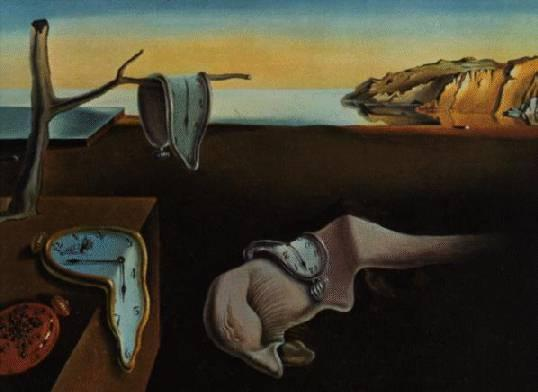
\includegraphics{jsslogo}
\caption{\label{fig:quine} Frequency distribution for number of days absent
from school.}
\end{figure}

























%% -- Summary/conclusions/discussion -------------------------------------------

\section{Summary and discussion} \label{sec:summary}

\begin{leftbar}
As usual \dots
\end{leftbar}

























%% -- Optional special unnumbered sections -------------------------------------

\section*{Computational details}

\begin{leftbar}
If necessary or useful, information about certain computational details
such as version numbers, operating systems, or compilers could be included
in an unnumbered section. Also, auxiliary packages (say, for visualizations,
maps, tables, \dots) that are not cited in the main text can be credited here.
\end{leftbar}

The results in this paper were obtained using
\proglang{R}~3.4.1 with the
\pkg{MASS}~7.3.47 package. \proglang{R} itself
and all packages used are available from the Comprehensive
\proglang{R} Archive Network (CRAN) at
\url{https://CRAN.R-project.org/}.


\section*{Acknowledgments}

\begin{leftbar}
All acknowledgments (note the AE spelling) should be collected in this
unnumbered section before the references. It may contain the usual information
about funding and feedback from colleagues/reviewers/etc. Furthermore,
information such as relative contributions of the authors may be added here
(if any).
\end{leftbar}

 
\newpage
%% -- Bibliography -------------------------------------------------------------
%% - References need to be provided in a .bib BibTeX database.
%% - All references should be made with \cite, \citet, \citep, \citealp etc.
%%   (and never hard-coded). See the FAQ for details.
%% - JSS-specific markup (\proglang, \pkg, \code) should be used in the .bib.
%% - Titles in the .bib should be in title case.
%% - DOIs should be included where available.

\bibliography{../../bibliografia/journalsAbbr,../../bibliografia/Gaming/gaming}

\newpage

\begin{appendix}











































































































\newpage

\section{Propiedades}\label{sec:propiedades}

Las siguientes tres propiedades, junto con las reglas del \emph{sum-product algorithm}, es lo \'unico que se necesita para calcular la posterior anal\'itica del modelo bayesiano.

\subsection*{Multiplicacion de normales}
\begin{equation}\label{eq:multiplicacion_normales}
\begin{split}
 \int_{-\infty}^{\infty} N(x|\mu_x,\sigma_x^2)N(x|\mu_y,\sigma_y^2) \, dx  &  \overset{*}{=} \int_{-\infty}^{\infty}  \underbrace{N(\mu_x|\mu_y,\sigma_x^2+\sigma_y^2)}_{\text{constante}} N(x|\mu_{*},\sigma_{*}^2) dx \\
 & = N(\mu_x|\mu_y,\sigma_x^2+\sigma_y^2) \underbrace{\int_{-\infty}^{\infty}  N(x|\mu_{*},\sigma_{*}^2) dx}_{1} \\
 & = N(\mu_x|\mu_y,\sigma_x^2+\sigma_y^2)
\end{split}
\end{equation}

Donde la igualdad destacada ($\overset{*}{=}$) se demuestra en la secci\'on~\ref{multiplicacion_normales} anexa.

\subsection*{Integrales con funci\'on indicadora}
\begin{equation}\label{eq:integral_con_indicadora}
\begin{split}
 \int_{-\infty}^{\infty}  \int_{-\infty}^{\infty}  \mathbb{I}(x=h(y,z)) f(x) g(y)\, dx\, dy &=  \int_{-\infty}^{\infty} \int_{h(y,z)}^{h(y,z)} f(h(y,z)) g(y)\, dx\, dy\\
 & = \int_{-\infty}^{\infty} f(h(y,z)) g(y) dy
 %& \propto \int f(h(y,z)) g(y) dy
\end{split}
\end{equation}

\subsection*{Simetr\'ia de normales}
\begin{equation}\label{eq:simetria}
 N(x|\mu,\sigma^2) = N(\mu|x,\sigma^2) = N(-\mu|-x,\sigma^2) = N(-x|-\mu,\sigma^2)
\end{equation}

\subsection*{Derivada de la acumulada normal}
\begin{equation}\label{eq:phi_norm}
 \frac{\partial}{\partial x} \Phi(x|\mu,\sigma^2) = N(x|\mu,\sigma^2)
\end{equation}

\subsection*{Distribuci\'on normal estandarizada}
\begin{equation}\label{eq:estandarizar}
 X \sim N(\mu,\sigma^2) \Rightarrow \frac{X-\mu}{\sigma} \sim N(0,1)
\end{equation}



\section{Ejemplo 2 vs 2}

\begin{figure}[t!]
  \centering
  \scalebox{.75}{\tikz{ %
        
      
        \node[factor] (fr) {} ;
        \node[const, right=of fr] (nfr) {$f_{r_1}$}; %
	
	\node[latent, above=of fr] (d) {$d_1$} ; %
        \node[factor, above=of d] (fd) {} ;
        \node[const, right=of fd] (nfd) {$f_{d_1}$}; %
	
        
        \node[latent, above=of fd,xshift=-0.75cm] (ta) {$t_a$} ; %
        \node[factor, left=of ta] (fta) {} ;
        \node[const, above=of fta] (nfta) {$f_{t_a}$}; %
        
        
        
        \node[latent, left=of fta,yshift=1cm] (p1) {$p_1$} ; %
        \node[factor, left=of p1] (fp1) {} ;
        \node[const, above=of fp1] (nfp1) {$f_{p_1}$}; %
        
        \node[latent, left=of fp1] (s1) {$s_1$} ; %
        \node[factor, left=of s1] (fs1) {} ;
	\node[const, above=of fs1] (nfs1) {$f_{s_1}$}; %
     
        \node[latent, left=of fta,yshift=-1cm] (p2) {$p_2$} ; %
        \node[factor, left=of p2] (fp2) {} ;
        \node[const, above=of fp2] (nfp2) {$f_{p_2}$}; %
        
        \node[latent, left=of fp2] (s2) {$s_2$} ; %
        \node[factor, left=of s2] (fs2) {} ;
	\node[const, above=of fs2] (nfs2) {$f_{s_2}$}; %
        
            
        \node[latent, above=of fd,xshift=0.75cm] (tb) {$t_b$} ; %
        \node[factor, right=of tb] (ftb) {} ;
        \node[const, above=of ftb] (nftb) {$f_{t_b}$}; %
        
        \node[latent, right=of ftb,yshift=1cm] (p3) {$p_3$} ; %
        \node[factor, right=of p3] (fp3) {} ;
        \node[const, above=of fp3] (nfp3) {$f_{p_3}$}; %
        
        \node[latent, right=of fp3] (s3) {$s_3$} ; %
        \node[factor, right=of s3] (fs3) {} ;
	\node[const, above=of fs3] (nfs3) {$f_{s_3}$}; %
     
        \node[latent, right=of ftb,yshift=-1cm] (p4) {$p_4$} ; %
        \node[factor, right=of p4] (fp4) {} ;
        \node[const, above=of fp4] (nfp4) {$f_{p_4}$}; %
        
        \node[latent, right=of fp4] (s4) {$s_4$} ; %
        \node[factor, right=of s4] (fs4) {} ;
	\node[const, above=of fs4] (nfs4) {$f_{s_4}$}; %
     
        \edge[-] {fr} {d};
	\edge[-] {d} {fd};
	
        \edge[-] {fd} {ta};
        \edge[-] {ta} {fta};
        \edge[-] {fta} {p1};
        \edge[-] {p1} {fp1};
        \edge[-] {fp1} {s1};
        \edge[-] {s1} {fs1};
        \edge[-] {fta} {p2};
        \edge[-] {p2} {fp2};
        \edge[-] {fp2} {s2};
        \edge[-] {s2} {fs2};
        	
	\edge[-] {fd} {tb};
        \edge[-] {tb} {ftb};
        \edge[-] {ftb} {p3};
        \edge[-] {p3} {fp3};
        \edge[-] {fp3} {s3};
        \edge[-] {s3} {fs3};
        \edge[-] {ftb} {p4};
        \edge[-] {p4} {fp4};
        \edge[-] {fp4} {s4};
        \edge[-] {s4} {fs4};
        
	
	\node[const, below=of nfr,xshift=7cm,yshift=-1cm] (dfr) { $fr_1 = \mathbb{I}(d_1>0)$}; %
	\node[const, left=of dfr,xshift=-0.5cm] (dfd) {$fd_1 = \mathbb{I}(d_1=t_a - t_b)$}; %
	\node[const, left=of dfd,xshift=-0.5cm] (dft) {$ft_e = \mathbb{I}(t_e = \sum_{i \in A_e} p_i)$}; %
        \node[const, left=of dft,xshift=-0.5cm] (dfp) {$fp_i = N(p_i;s_i,\beta^2)$}; %
        \node[const, left=of dfp,xshift=-0.5cm] (dfs) {$fs_i = N(s_i;\mu_i,\sigma^2)$}; %
 
	
	%\node[const, right= of r, xshift=1.2cm ,yshift=-2.1cm] (result-dist) {$r_{ab} \sim B\left(\Phi\left(\frac{\mu_a - \mu_b}{\sqrt{\beta_a^2+\beta_b^2}}\right)\right)$} ; %
	      
        }}
  \caption{\small Grafo bipartito de factorizaci\'on del modelo \texttt{TrueSkill} (Caso 2 vs 2)}
  \label{modelo_trueskill_2vs2}
\end{figure}


\subsection{Mensajes descendentes}

\paragraph{$\bm{m_{f_s \rightarrow s}(s)}:$}

\begin{equation}\label{eq:m_fs_s}
\begin{split}
 m_{f_{s_i} \rightarrow s_i}(s_i) & \overset{\hfrac{\text{eq}}{\ref{eq:m_f_v}}}{=} \int \dots \int f_{s_i}(\bm{x}) \prod_{h \in n(f_{s_i}) \setminus \{s_i\} } m_{h \rightarrow f_{s_i}}(h) d\bm{x}_{\setminus \{s_i\}}  \\
& \overset{\hfrac{\text{fig}}{\ref{modelo_trueskill_2vs2}}}{=} \int \dots \int N(s_i| \mu_i, \sigma_i^2) d\bm{x}_{\setminus \{s_i\} } \\
& \underset{*}{\overset{\hfrac{\text{eq}}{\ref{eq:m_f_v}}}{=}} N(s_i| \mu_i, \sigma_i^2)
\end{split}
\end{equation}

Notar que la igualdad se\~nalada $\overset{*}{=}$ vale por definici\'on de la notaci\'on resumen (Eq.~\ref{eq:m_f_v}),

\begin{equation*}
\begin{split}
\bm{x}_{\setminus \{s_i\} } & = \text{arg}(f) \setminus \{s_i\} \\
&= \text{arg}(N(s_i| \mu_i, \sigma_i^2)) \setminus \{s_i\} \\
&= \{s_i\} \setminus \{s_i\} \\
& = \emptyset
\end{split}
\end{equation*}



\paragraph{$\bm{m_{s \rightarrow f_p}(s)}:$}

\begin{equation}\label{eq:m_s_fp}
 m_{s_i \rightarrow f_{p_i}}(s_i) \overset{\hfrac{\text{eq}}{\ref{eq:m_v_f}}}{=} \prod_{g \in n(s_i) \setminus  \{f_{p_i} \}} m_{g \rightarrow s_i} (s_i) \overset{\hfrac{\text{fig}}{\ref{modelo_trueskill_2vs2}}}{=} m_{f_{s_i} \rightarrow s_i}(s_i) \overset{\hfrac{\text{eq}}{\ref{eq:m_fs_s}}}{=}   N(s_i| \mu_i, \sigma_i^2)
\end{equation}



\paragraph{$\bm{m_{f_p \rightarrow p}(p)}:$}

\begin{equation}\label{eq:m_fp_p}
\begin{split}
 m_{f_{p_i} \rightarrow p_i}(p_i) & \overset{\hfrac{\text{eq}}{\ref{eq:m_f_v}}}{=} \int \dots \int f_{p_i}(\bm{x}) \prod_{h \in n(f_{p_i}) \setminus \{p_i\} } m_{h \rightarrow f_{p_i}}(h) d\bm{x}_{\setminus \{p_i\} }  \\
 & \overset{\hfrac{\text{fig}}{\ref{modelo_trueskill_2vs2}}}{\underset{\hfrac{\text{eq}}{\ref{eq:m_s_fp}}}{=}} \int \dots \int N(p_i| s_i, \beta^2) N(s_i| \mu_i, \sigma_i^2) d\bm{x}_{\setminus \{p_i\} } \\[0.3cm]
 & \overset{\hfrac{\text{eq}}{\ref{eq:m_f_v}}}{=} \int N(p_i| s_i, \beta^2) N(s_i| \mu_i, \sigma_i^2) ds_i \\
 & \overset{\hfrac{\text{eq}}{\ref{eq:simetria}}}{=} \int N(s_i|p_i, \beta^2) N(s_i| \mu_i, \sigma_i^2) ds_i \\
& \overset{\hfrac{\text{eq}}{\ref{eq:multiplicacion_normales}}}{=} N(p_i|\mu_i,\beta^2 + \sigma_i^2)
\end{split}
\end{equation}

\paragraph{$\bm{m_{p \rightarrow f_t}(p)}:$}

\begin{equation}\label{eq:m_p_ft}
\begin{split}
 m_{p_i \rightarrow f_{t_e}}(p_i) & \overset{\hfrac{\text{eq}}{\ref{eq:m_v_f}}}{=} \prod_{g \in n(p_i) \setminus  \{f_{t_e} \}} m_{g \rightarrow p_i} (p_i) \\
 & \overset{\hfrac{\text{fig}}{\ref{modelo_trueskill_2vs2}}}{=} m_{f_{p_i} \rightarrow p_i}(p_i) \overset{\hfrac{\text{eq}}{\ref{eq:m_fp_p}}}{=} N(p_i|\mu_i,\beta^2 + \sigma_i^2)
\end{split}
\end{equation}

\paragraph{$\bm{m_{f_t \rightarrow t}(t)}:$}

\begin{equation}
\begin{split}
 m_{f_{t_e} \rightarrow t_e}(t_e) & \overset{\hfrac{\text{eq}}{\ref{eq:m_f_v}}}{=} \int \dots \int f_{t_e}(\bm{x}) \prod_{h \in n(f_{t_e}) \setminus \{t_e\} } m_{h \rightarrow f_{t_e}}(h) d\bm{x}_{\setminus \{t_e\} }  \\
 & \overset{\hfrac{\text{fig}}{\ref{modelo_trueskill_2vs2}}}{\underset{\hfrac{\text{eq}}{\ref{eq:m_p_ft}}}{=}} \int \dots \int \mathbb{I}(t_e = p_i + p_j) N(p_i|\mu_i,\beta^2 + \sigma_i^2)N(p_j|\mu_j,\beta^2 + \sigma_j^2) d\bm{x}_{\setminus \{t_e\} }\\[0.3cm]
 & \overset{\hfrac{\text{eq}}{\ref{eq:m_f_v}}}{=} \iint \mathbb{I}(t_e = p_i + p_j) N(p_i|\mu_i,\beta^2 + \sigma_i^2)N(p_j|\mu_j,\beta^2 + \sigma_j^2) dp_idp_j \\
 & \overset{\hfrac{\text{eq}}{\ref{eq:integral_con_indicadora}}}{=} \int N(p_i|\mu_i,\beta^2 + \sigma_i^2) N(t_e - p_i|\mu_j,\beta^2 + \sigma_j^2) dp_i   \\
 & \overset{\hfrac{\text{eq}}{\ref{eq:simetria}}}{=} \int N(p_i|\mu_i,\beta^2 + \sigma_i^2) N(p_i|t_e - \mu_j,\beta^2 + \sigma_j^2) dp_i \\
 & \overset{\hfrac{\text{eq}}{\ref{eq:multiplicacion_normales}}}{=} N(t_e|\mu_i+\mu_j,2\beta^2 + \sigma_i^2 + \sigma_j^2)
\end{split}
\end{equation}

\vspace{0.3cm}

General (por inducci\'on)
\begin{equation}\label{eq:m_ft_t}
 m_{f_{t_e} \rightarrow t_e}(t_e) =  N \Big( t_e | \underbrace{\sum_{i\in A_e } \mu_i}_{\hfrac{\text{Habilidad}}{\text{de equipo}} \ \mu_e}, \underbrace{\sum_{i \in A_e} \beta^2 + \sigma_i^2}_{\hfrac{\text{Varianza}}{\text{de equipo}} \ \sigma_e^2} \Big) = N(t_e | \mu_e, \sigma_e^2)
\end{equation}

Ver anexo~\ref{suma_normales_induccion}, la secci\'on sobre suma de $n$ normales.

\paragraph{$\bm{m_{t \rightarrow f_d}(t)}:$}

\begin{equation}\label{eq:m_t_fd}
\begin{split}
m_{t_e \rightarrow f_{d_{k}}}(d_{k}) & \overset{\hfrac{\text{eq}}{\ref{eq:m_v_f}}}{=} \prod_{g \in n(t_e) \setminus  \{f_{d_{k}} \}} m_{g \rightarrow t_e} (t_e) \\[0.3cm]
 & \overset{\hfrac{\text{fig}}{\ref{modelo_trueskill_2vs2}}}{=} m_{f_{t_e} \rightarrow t_e}(t_e) \overset{\hfrac{\text{eq}}{\ref{eq:m_ft_t}}}{=} N(t_e| \sum_{i \in A_e} \mu_i, \sum_{i \in A_e} \beta^2 + \sigma_i^2) \overset{\hfrac{\text{eq}}{\ref{eq:m_ft_t}}}{=} N(t_e|\mu_e,\sigma_e^2)
\end{split}
\end{equation}

\paragraph{$\bm{m_{f_d \rightarrow d}(d)}:$}

\begin{equation}
 \begin{split}
  m_{f_{d_1} \rightarrow d_1}(d_1) & \overset{\hfrac{\text{eq}}{\ref{eq:m_f_v}}}{=} \int \dots \int f_{d_1}(\bm{x}) \prod_{h \in n(f_{d_1}) \setminus \{d_1\} } m_{h \rightarrow f_{d_1}}(h) \, d\bm{x}_{\setminus \{d_1\} }  \\
  & \overset{\hfrac{\text{fig}}{\ref{modelo_trueskill_2vs2}}}{\underset{\hfrac{\text{eq}}{\ref{eq:m_t_fd}}}{=}} \int \int \mathbb{I}(d_1 = t_a - t_b) N(t_a| \mu_a, \sigma_a^2)  N(t_b| \mu_b, \sigma_b^2)  dt_adt_b \\[0.25cm]
  & \overset{\hfrac{\text{eq}}{\ref{eq:integral_con_indicadora}}}{=} \int N(d_1 + t_b| \mu_a, \sigma_a^2)  N(t_b| \mu_a, \sigma_b^2)  dt_b \\
  & \overset{\hfrac{\text{eq}}{\ref{eq:simetria}}}{=} \int N(t_b| \mu_a - d_1 , \sigma_a^2)  N(t_b| \mu_b, \sigma_b^2)  dt_b \\
  & \overset{\hfrac{\text{eq}}{\ref{eq:multiplicacion_normales}}}{=} N( \mu_a - d_1 | \mu_b, \sigma_a^2 +\sigma_b^2  ) \\
  & \overset{\hfrac{\text{eq}}{\ref{eq:simetria}}}{=} N( d_1 | \mu_a - \mu_b, \sigma_a^2 +\sigma_b^2  )
 \end{split}
\end{equation}

General

\begin{equation} \label{eq:m_fd_d}
 m_{f_{d_1} \rightarrow d_1}(d_1) = N\Bigg(d_1 \ | \ \underbrace{\sum_{i \in A_a} \mu_i - \sum_{i \in A_b} \mu_i}_{\hfrac{\text{Diferencia}}{\text{esperada}} \, (\delta)} \ , \  \underbrace{\sum_{i \in A_a \cup A_b} \beta^2 + \sigma_i^2}_{\hfrac{\text{Varianza}}{\text{total}} \, (\vartheta) } \Bigg) = N(d_1 | \delta, \vartheta)
\end{equation}

\paragraph{$\bm{m_{d \rightarrow f_r}(r)}:$}

\begin{equation}\label{eq:m_d_fr}
\begin{split}
m_{d \rightarrow f_r}(d) & \overset{\hfrac{\text{eq}}{\ref{eq:m_v_f}}}{=} \prod_{g \in n(t_e) \setminus  \{f_{d_{k}} \}} m_{g \rightarrow t_e} (t_e) \\[0.3cm]
 & \overset{\hfrac{\text{fig}}{\ref{modelo_trueskill_2vs2}}}{=} m_{f_d \rightarrow d}(d) \overset{\hfrac{\text{eq}}{\ref{eq:m_fd_d}}}{=} N(d_1| \delta, \vartheta)
\end{split}
\end{equation}

\paragraph{$\bm{m_{f_r \rightarrow r}(r)}:$} (Caso ganador)

\begin{equation}\label{eq:m_fr_r}
\begin{split}
 m_{f_{r_1} \rightarrow r_1}(r_1) & \overset{\hfrac{\text{eq}}{\ref{eq:m_f_v}}}{=} \int \dots \int f_{r_1}(\bm{x}) \prod_{h \in n(f_{r_1}) \setminus \{r_1\} } m_{h \rightarrow f_{r_1}}(h) \, d\bm{x}_{\setminus \{r_1\} }  \\[0.2cm]
 & \overset{\hfrac{\text{fig}}{\ref{modelo_trueskill_2vs2}}}{\underset{\hfrac{\text{eq}}{\ref{eq:m_d_fr}}}{=}} \int \mathbb{I}(d_1 > 0) N(d_1 | \delta, \vartheta)  dd_1 \\[0.2cm]
 &  \overset{\hfrac{\text{eq}}{\ref{eq:estandarizar}}}{=} \int \mathbb{I}(d_1 > 0) N( \frac{d_1 - \delta}{\vartheta}) dd_1 \\[0.2cm]
 & = 1 - \Phi(\frac{-\delta}{\vartheta}) \\
 & = \Phi(\frac{\delta}{\vartheta})
\end{split}
\end{equation}













\subsubsection{Mensajes ascendentes}

\paragraph{$\bm{m_{f_r \rightarrow d}(d)}:$}

\begin{equation}\label{eq:m_fr_d}
\begin{split}
m_{f_r \rightarrow d_1}(d_1) & \overset{\hfrac{\text{fig}}{\ref{modelo_trueskill_2vs2}}}{\underset{\hfrac{\text{eq}}{\ref{eq:m_f_v}}}{=}} \mathbb{I}(d_1 > 0)
\end{split}
\end{equation}


\paragraph{$\bm{m_{d \rightarrow f_d}(d)}:$}
\begin{equation}\label{eq:m_d_fd}
\begin{split}
m_{d_1 \rightarrow f_{d_1}}(d_1) & \overset{\hfrac{\text{eq}}{\ref{eq:m_v_f}}}{=} \prod_{g \in n(d_1) \setminus  \{f_{d_1} \}} m_{g \rightarrow d_1} (d_1) \\[0.3cm]
 & \overset{\hfrac{\text{fig}}{\ref{modelo_trueskill_2vs2}}}{=} m_{f_r \rightarrow d_1}(d_1) \overset{\hfrac{\text{eq}}{\ref{eq:m_fr_d}}}{=} \mathbb{I}(d_1 > 0)
\end{split}
\end{equation}

\paragraph{$\bm{m_{f_{d_1} \rightarrow t_a}(t_a)}:$} (Caso ganador)
\begin{equation}\label{eq:m_fd_ta}
\begin{split}
m_{f_{d_1} \rightarrow t_a}(t_a) & \overset{\hfrac{\text{eq}}{\ref{eq:m_f_v}}}{=} \int \dots \int f_{d_1}(\bm{x}) \prod_{h \in n(f_{d_1}) \setminus \{t_a\} } m_{h \rightarrow f_{d_1}}(h) \, d\bm{x}_{\setminus \{t_a\} }  \\
&\overset{\hfrac{\text{fig}}{\ref{modelo_trueskill_2vs2}}}{\underset{\hfrac{\text{eq}}{\ref{eq:m_t_fd}}}{=}}  \int \dots \int \mathbb{I}(d_1 = t_a - t_b) \mathbb{I}(d_1 > 0) N(t_b | \mu_b , \sigma_b^2 )  \, d\bm{x}_{\setminus \{t_a\} } \\[0.1cm]
& \overset{\hfrac{\text{eq}}{\ref{eq:m_f_v}}}{=} \iint \mathbb{I}(d_1 = t_a - t_b) \mathbb{I}(d_1 > 0) N(t_b | \mu_b , \sigma_b^2 ) \, dd_1\,dt_b \\
& \overset{\hfrac{\text{eq}}{\ref{eq:integral_con_indicadora}}}{=} \int \mathbb{I}( t_a > t_b)  N(t_b | \mu_b , \sigma_b^2 ) \,dt_b  \\
& \overset{\hfrac{\text{fig}}{\ref{fig:m_fd_t}}}{=} \Phi (t_a| \mu_b, \sigma_b^2)  \overset{\hfrac{\mu_b}{\sigma_b}}{=}  \Phi \Big(t_a| \sum_{i \in A_b} \mu_i , \sum_{i \in A_b} \beta^2 + \sigma_i^2 \Big)
\end{split}
\end{equation}

\paragraph{$\bm{m_{f_{d_1} \rightarrow t_b}(t_b)}:$} (Caso perdedor)
\begin{equation}\label{eq:m_fd_tb}
\begin{split}
m_{f_{d_1} \rightarrow t_b}(t_b) &\overset{\hfrac{\text{eq}}{\ref{eq:m_f_v}}}{=} \int \dots \int f_{d_1}(\bm{x}) \prod_{h \in n(f_{d_1}) \setminus \{t_b\} } m_{h \rightarrow f_{d_1}}(h) \, d\bm{x}_{\setminus \{t_a\} }  \\
&\overset{\hfrac{\text{fig}}{\ref{modelo_trueskill_2vs2}}}{\underset{\hfrac{\text{eq}}{\ref{eq:m_t_fd}}}{=}}  \int \dots \int \mathbb{I}(d_1 = t_a - t_b) \mathbb{I}(d_1 > 0) N(t_a | \mu_a , \sigma_a^2 )  \, d\bm{x}_{\setminus \{t_b\} } \\[0.1cm]
&\overset{\hfrac{\text{eq}}{\ref{eq:m_f_v}}}{=} \iint \mathbb{I}(d_1 = t_a - t_b) \mathbb{I}(d_1 > 0)  N(t_a | \mu_a , \sigma_a^2 )  \, dd_1\,dt_a \\
&\overset{\hfrac{\text{eq}}{\ref{eq:integral_con_indicadora}}}{=} \int \mathbb{I}( t_a > t_b)   N(t_a | \mu_a , \sigma_a^2 ) \,dt_a \\
&\overset{\hfrac{\text{fig}}{\ref{fig:m_fd_t}}}{=} 1 - \Phi (t_b| \mu_a , \sigma_a^2 ) \overset{\hfrac{\mu_a}{\sigma_a}}{=} 1 - \Phi \Big(t_b| \sum_{i \in A_a} \mu_i , \sum_{i \in A_a} \beta^2 + \sigma_i^2 \Big)
\end{split}
\end{equation}

\begin{figure}[t!]
\centering
  \begin{subfigure}[t]{0.48\textwidth}
  \includegraphics[width=\textwidth]{figures/m_d_ta.pdf}
  \caption{$m_{f_{d_1} \rightarrow t_a}(t_a)$: (Caso ganador)}
  \label{fig:m_fd_ta}
  \end{subfigure}
  \begin{subfigure}[t]{0.48\textwidth}
  \includegraphics[width=\textwidth]{figures/m_d_tb.pdf}
  \caption{$m_{f_{d_1} \rightarrow t_b}(t_b)$: (Caso perdedor)}
  \label{fig:m_fd_tb}
  \end{subfigure}
  \caption{Notar que en el caso ganador, $t_a$ es un valor fijo que entra como par\'ametro en la funci\'on $m_{f_{d_1} \rightarrow t_a}(t_a)$. El caso perdedor es an\'alogo.}
  \label{fig:m_fd_t}
\end{figure}

\paragraph{$\bm{m_{t_a \rightarrow f_{t_a}}(t_a)}:$} (Caso ganador)

\begin{equation}\label{eq:m_ta_ft}
\begin{split}
 m_{t_a \rightarrow f_{t_a}}(t_a) \overset{\hfrac{\text{eq}}{\ref{eq:m_v_f}}}{=} \prod_{g \in n(t_a) \setminus  \{f_{t_a} \}} m_{g \rightarrow t_a} (t_a)  \overset{\hfrac{\text{eq}}{\ref{eq:m_fd_ta}}}{=} \Phi(t_a|\mu_b,\sigma_b^2) \overset{\hfrac{\mu_b}{\sigma_b}}{=} \Phi \Big(t_a| \sum_{i \in A_b} \mu_i , \sum_{i \in A_b} \beta^2 + \sigma_i^2 \Big)
\end{split}
\end{equation}

\paragraph{$\bm{m_{t_b \rightarrow f_{t_b}}(t_b)}:$} (Caso perdedor)
\begin{equation}\label{eq:m_tb_ft}
\begin{split}
 m_{t_b \rightarrow f_{t_b}}(t_b) \overset{\hfrac{\text{eq}}{\ref{eq:m_v_f}}}{=} \prod_{g \in n(t_b) \setminus  \{f_{t_b} \}} m_{g \rightarrow t_b} (t_b)  \overset{\hfrac{\text{eq}}{\ref{eq:m_fd_tb}}}{=} 1- \Phi(t_b|\mu_a,\sigma_a^2) \overset{\hfrac{\mu_a}{\sigma_a}}{=} 1 - \Phi \Big(t_b| \sum_{i \in A_a} \mu_i , \sum_{i \in A_a} \beta^2 + \sigma_i^2 \Big)
\end{split}
\end{equation}



\paragraph{$\bm{m_{f_{t_a} \rightarrow p_1}(p_1)}:$} (Caso ganador)
\begin{equation}\label{eq:m_fta_p_inicial}
\begin{split}
m_{f_{t_a} \rightarrow p_1}(p_1)  &\overset{\hfrac{\text{eq}}{\ref{eq:m_f_v}}}{=} \int \dots \int f_{t_a}(\bm{x}) \prod_{h \in n(f_{t_a}) \setminus \{p_1\} } m_{h \rightarrow f_{t_a}}(h) \, d\bm{x}_{\setminus \{p_1\} }  \\
&\overset{\hfrac{\text{fig}}{\ref{modelo_trueskill_2vs2}}}{\underset{\hfrac{\text{eq}}{\ref{eq:m_ta_ft}}}{=}} \int \dots \int \mathbb{I}( t_a = p_1 + p_2) N(p_2| \mu_2, \beta^2 + \sigma_2^2 ) \, \Phi (t_a| \mu_b , \sigma_b^2 ) \, d\bm{x}_{\setminus \{p_1\} }\\[0.1cm]
&\overset{\hfrac{\text{eq}}{\ref{eq:m_f_v}}}{=} \iint \mathbb{I}( t_a = p_1 + p_2) \, N(p_2| \mu_2, \beta^2 + \sigma_2^2 ) \, \Phi (t_a| \mu_b , \sigma_b^2 ) \, dt_a dp_2 \\
&\overset{\hfrac{\text{eq}}{\ref{eq:integral_con_indicadora}}}{=} \int  \, N(p_2| \mu_2, \beta^2 + \sigma_2^2 ) \, \Phi (p_1 + p_2| \mu_b , \sigma_b^2 ) \, dp_2 \\
&\overset{\hfrac{\text{eq}}{\ref{eq:simetria}}}{=} \int  N(p_2| \mu_2, \beta^2 + \sigma_2^2 ) \, \Phi (p_1 | \mu_b - p_2 , \sigma_b^2) \, dp_2 \\
&= \kappa(p_1)
\end{split}
\end{equation}

La derivada de la funci\'on de distribuci\'on acumulada $\Phi(\,)$ es el valor de la densidad de la funci\'on de probabilidad $N(\,)$. Con esta idea en mente, tomamos la derivada de ambos lados de la igualdad:

\begin{equation}\label{eq:ta-p_derivada}
\begin{split}
\frac{\partial\kappa(x)}{\partial x} &= \frac{\partial}{\partial x} \int  N(y| \mu_y, \sigma_y^2 ) \,   \Phi (x | \mu_x -y , \sigma_x^2 ) \, dy \\
&= \int  N(y| \mu_y, \sigma_y^2 ) \, \frac{\partial}{\partial x} \,\Phi (x| \mu_x - y, \sigma_x^2 )  \, dy   \\
& \overset{\hfrac{\text{eq}}{\ref{eq:phi_norm}}}{=} \int  N(y| \mu_y, \sigma_y^2 ) \, N(x| \mu_x -y , \sigma_x^2)  \, dy  \\
& \overset{\hfrac{\text{eq}}{\ref{eq:simetria}}}{=} \int  N(y| \mu_y, \sigma_y^2 ) \, N(y| \mu_x  -x , \sigma_x^2)  \, dy  \\
&\overset{\hfrac{\text{eq}}{\ref{eq:multiplicacion_normales}}}{\underset{\hfrac{\text{eq}}{\ref{eq:simetria}}}{=}} N(x| \mu_x - \mu_y, \sigma_x^2 + \sigma_y^2)
\end{split}
\end{equation}

Luego

\begin{equation}\label{eq:m_fta_p}
 m_{f_{t_a} \rightarrow p_1}(p_1) \overset{\hfrac{\text{eq}}{\ref{eq:m_fta_p_inicial}}}{\underset{\hfrac{\text{eq}}{\ref{eq:ta-p_derivada}}}{=}}  \Phi(p_1| \mu_b - \mu_2, \beta^2 + \sigma_2^2 + \sigma_b^2)  \overset{\hfrac{\mu_b}{\sigma_b}}{=}  \Phi\Big(p_1| \sum_{i \in A_b} \mu_i - \mu_2, \beta^2 + \sigma_2^2 + \sum_{i \in A_b} \beta^2 + \sigma_i^2 \Big)
\end{equation}

\paragraph{$\bm{m_{f_{t_b} \rightarrow p_3}(p_3)}:$} (Caso perdedor)
\begin{equation}\label{eq:m_ftb_p}
\begin{split}
m_{f_{t_b} \rightarrow p_3}(p_3)&\overset{\hfrac{\text{eq}}{\ref{eq:m_f_v}}}{=} \int \dots \int f_{t_a}(\bm{x}) \prod_{h \in n(f_{t_a}) \setminus \{p_1\} } m_{h \rightarrow f_{t_a}}(h) \, d\bm{x}_{\setminus \{p_1\} }  \\
&\overset{\hfrac{\text{fig}}{\ref{modelo_trueskill_2vs2}}}{\underset{\hfrac{\text{eq}}{\ref{eq:m_tb_ft}}}{=}} \int \dots \int \mathbb{I}( t_b = p_3 + p_4) \, (1-\Phi (t_b| \mu_a , \sigma_a^2 )) \, N(p_4| \mu_4, \beta^2 + \sigma_4^2 ) \, d\bm{x}_{\setminus \{p_3\} }\\[0.1cm]
&\overset{\hfrac{\text{eq}}{\ref{eq:m_f_v}}}{=} \iint \mathbb{I}( t_b = p_3 + p_4) N(p_4| \mu_4, \beta^2 + \sigma_4^2 )  (1 - \Phi (t_b| \mu_a , \sigma_a^2) )\, dt_b dp_4 \\
&\overset{\hfrac{\text{eq}}{\ref{eq:integral_con_indicadora}}}{\underset{\hfrac{\text{eq}}{\ref{eq:simetria}}}{=}} \int N(p_4| \mu_4, \beta^2 + \sigma_4^2 )  (1 - \Phi (p_3 | \mu_a - p_4 , \sigma_a^2 ) ) \,  dp_4 \\
& =  \underbrace{\int N(p_4| \mu_4, \beta^2 + \sigma_4^2 )dp_4}_{1}  -  \underbrace{\int N(p_4| \mu_4, \beta^2 + \sigma_4^2 ) \Phi (p_3 | \mu_a - p_4 , \sigma_a^2 ) ) \, dp_4}_{\kappa(p_3)} \\
&\overset{\hfrac{\text{eq}}{\ref{eq:ta-p_derivada}}}{=} 1 - \Phi(p_3, \mu_a  - \mu_4, \beta^2 + \sigma_4^2 + \sigma_a^2)\\[0.1cm]
&\overset{\hfrac{\mu_a}{\sigma_a}}{=} 1 - \Phi\Big(p_3, \sum_{i \in A_a} \mu_i  - \mu_4, \beta^2 + \sigma_4^2 + \sum_{i \in A_a} \beta^2 + \sigma_i^2  \Big)
\end{split}
\end{equation}

\paragraph{$\bm{m_{p_1 \rightarrow f_{p_1}}(s_1)}:$} (Caso ganador)

\begin{equation}\label{eq:m_p1_fp}
\begin{split}
 m_{p_1 \rightarrow f_{p_1}}(p_1) \overset{\hfrac{\text{eq}}{\ref{eq:m_v_f}}}{=} \prod_{g \in n(p_1) \setminus  \{f_{p_1} \}} m_{g \rightarrow p_1} (p_1)  \overset{\hfrac{\text{eq}}{\ref{eq:m_fta_p}}}{=}  \Phi(p_1| \mu_b - \mu_2, \beta^2 + \sigma_2^2 + \sigma_b^2)
\end{split}
\end{equation}


\paragraph{$\bm{m_{p_3 \rightarrow f_{p_3}}(s_1)}:$} (Caso perdedor)

\begin{equation}\label{eq:m_p3_fp}
\begin{split}
 m_{p_3 \rightarrow f_{p_3}}(p_3) \overset{\hfrac{\text{eq}}{\ref{eq:m_v_f}}}{=} \prod_{g \in n(p_3) \setminus  \{f_{p_3} \}} m_{g \rightarrow p_3} (p_3)  \overset{\hfrac{\text{eq}}{\ref{eq:m_ftb_p}}}{=}  1 - \Phi(p_3, \mu_a  - \mu_4, \beta^2 + \sigma_4^2 + \sigma_a^2)
\end{split}
\end{equation}

\paragraph{$\bm{m_{f_{p_1} \rightarrow s_1}(s_1)}:$} (Caso ganador)
\begin{equation}\label{eq:m_fp_s1}
\begin{split}
m_{f_{p_1} \rightarrow s_1}(s_1) & \overset{\hfrac{\text{eq}}{\ref{eq:m_f_v}}}{=} \int \dots \int f_{p_1}(\bm{x}) \prod_{h \in n(f_{p_1}) \setminus \{s_1\} } m_{h \rightarrow f_{p_1}}(h) \, d\bm{x}_{\setminus \{s_1\} }  \\
&\overset{\hfrac{\text{fig}}{\ref{modelo_trueskill_2vs2}}}{\underset{\hfrac{\text{eq}}{\ref{eq:m_p1_fp}}}{=}} \int \dots \int N(p_1| s_1, \beta^2) \, \Phi(p_1| \mu_b - \mu_2, \beta^2 + \sigma_2^2 + \sigma_b^2 ) \, d\bm{x}_{\setminus \{s_1\} }
\\[0.1cm]
& \overset{\hfrac{\text{eq}}{\ref{eq:m_f_v}}}{\underset{\hfrac{\text{eq}}{\ref{eq:simetria}}}{=}} \int N(p_1| s_1, \beta^2) \, \Phi(\mu_2| \mu_b -  p_1, \beta^2 + \sigma_2^2 + \sigma_b^2) \, dp_1 \\[0.1cm]
&\overset{\hfrac{\text{eq}}{\ref{eq:ta-p_derivada}}}{=} \Phi(s_1| \mu_b - \mu_2, 2\beta^2 + \sigma_2^2 + \sigma_b^2)
\end{split}
\end{equation}

General (N vs N)
\begin{equation}\label{eq:m_fp_s1_gral}
\begin{split}
m_{f_{p_1} \rightarrow s_1}(s_1) & \overset{\hfrac{\text{eq}}{\ref{eq:m_fp_s1}}}{=} \Phi(s_1| \mu_b - \mu_a + \mu_1, \sigma_b^2 +\sigma_a^2 - \sigma_1^2 )  \\
& \overset{\hfrac{\mu_b}{\sigma_b}}{=} \Phi\Big(s_1| \underbrace{\sum_{i \in A_b} \mu_i - \sum_{i \in A_a} \mu_i }_{-\hfrac{\text{Diferencia}}{\text{esperada}} \, -\delta = \delta } + \mu_1 , \underbrace{\sum_{i \in A_b \cup A_a} \beta^2 + \sigma_i^2}_{\hfrac{\text{Varianza}}{\text{total}} \, \vartheta^2} - \sigma_1^2   \Big) \\
& \overset{\hfrac{\delta}{\vartheta}}{=} \Phi(s_1|-\delta + \mu_1,\vartheta^2-\sigma_1^2) \\
& \overset{\hfrac{\text{eq}}{\ref{eq:simetria}}}{=} 1- \Phi(0| \underbrace{\delta - \mu_1 + s_1}_{\hfrac{\text{Diferencia esperada}}{\text{parametrizada}} \, \delta_1(s_1)},\underbrace{\vartheta^2-\sigma_1^2}_{\vartheta_1^2}) \\
& \overset{\hfrac{\delta_1}{\vartheta_1}}{=} 1- \Phi(0|\delta_1(s_1),\vartheta_1^2) \\
&\overset{\hfrac{\text{eq}}{\ref{eq:estandarizar}}}{=} 1- \Phi\Big(\frac{0-\delta_1(s_1)}{\vartheta_1}\Big)\\
&\overset{\hfrac{\text{eq}}{\ref{eq:simetria}}}{=} \Phi\Big(\frac{\delta_1(s_1)}{\vartheta_1}\Big)
\end{split}
\end{equation}

\textbf{Nota}: el mensaje $m_{f_{p_1} \rightarrow s_1}(s_1)$ computa la ``probabilidad de ganar parametrizada'', esto es la probabilidad de ganar si conoci\'eramos la habilidad del jugador. Si conocemos la habilidad del jugador entonces hay que eliminar la varianza de la distribuci\'on de creencias de la varianza total (lo que hacemos en $\vartheta_1$) y hay que remplazar la media de la distribuci\'on de creencias por la verdadera habilidad en la diferencia esperada (lo que hacemos en $\delta_1(s_1)$).

\paragraph{$\bm{m_{f_{p_3} \rightarrow s_3}(s_3)}:$}

\begin{equation}\label{eq:m_fp_s3}
\begin{split}
m_{f_{p_3} \rightarrow s_3}(s_3) & \overset{\hfrac{\text{eq}}{\ref{eq:m_f_v}}}{=} \int \dots \int f_{p_3}(\bm{x}) \prod_{h \in n(f_{p_3}) \setminus \{s_3\} } m_{h \rightarrow f_{p_3}}(h) \, d\bm{x}_{\setminus \{s_3\} }  \\
&\overset{\hfrac{\text{fig}}{\ref{modelo_trueskill_2vs2}}}{\underset{\hfrac{\text{eq}}{\ref{eq:m_p3_fp}}}{=}} \int \dots \int N(p_3| s_3, \beta^2) (1 - \Phi(p_3, \mu_a  - \mu_4, \beta^2 + \sigma_4^2 + \sigma_a^2)) \, d\bm{x}_{\setminus \{s_3\} }\\
& \overset{\hfrac{\text{eq}}{\ref{eq:m_f_v}}}{\underset{\hfrac{\text{eq}}{\ref{eq:simetria}}}{=}} \int N(p_3| s_3, \beta^2) (1 - \Phi(\mu_4, \mu_a  - p_3, \beta^2 + \sigma_4^2 + \sigma_a^2)) \, dp_3 \\
&=\int N(p_3| s_3, \beta^2) \, dp_3 -  \int N(p_3| s_3, \beta^2)  \Phi(\mu_4, \mu_a  - p_3, \beta^2 + \sigma_4^2 + \sigma_a^2) \, dp_3 \\
&\overset{\hfrac{\text{eq}}{\ref{eq:ta-p_derivada}}}{=} 1 - \Phi\Big(s_3| \mu_a-  \mu_4, 2\beta^2 + \sigma_4^2 + \sigma_a^2 \Big)
\end{split}
\end{equation}

General (N vs N)

\begin{equation}
\begin{split}
m_{f_{p_3} \rightarrow s_3}(s_3) & \overset{\hfrac{\text{eq}}{\ref{eq:m_fp_s3}}}{=} 1 - \Phi\Big(s_3| \underbrace{\mu_a-\mu_b}_{\delta}+\mu_3, \underbrace{\sigma_a^2 + \sigma_b^2}_{\vartheta^2} - \sigma_3^2 \Big) \\
& \overset{\hfrac{\delta}{\vartheta}}{=} 1 - \Phi\Big(s_3| \delta +\mu_3, \vartheta^2- \sigma_3^2 \Big) \overset{\hfrac{\text{eq}}{\ref{eq:simetria}}}{=} \Phi\Big(0| \underbrace{-\delta-\mu_3+s_3}_{\delta_3(s_3)}, \underbrace{\vartheta^2- \sigma_3^2}_{\vartheta_3^2} \Big) \\
& \overset{\hfrac{\delta_3}{\vartheta_3}}{=} \Phi(0|\delta_3(s_3),\vartheta_3^2)  \overset{\hfrac{\text{eq}}{\ref{eq:estandarizar}}}{=}  \Phi\left(\frac{0-\delta_3(s_3)}{\vartheta_3}\right) \\
& \overset{\hfrac{\text{eq}}{\ref{eq:simetria}}}{=} \Phi\Big(\frac{-\delta_3(s_3)}{\vartheta_3}\Big)
\end{split}
\end{equation}

\textbf{Nota}: el mensaje $m_{f_{p_3} \rightarrow s_3}(s_3)$ computa la ``probabilidad de perder parametrizada'' (que es la misma que la probabilidad de ganar de su contrincante). Si conoci\'eramos la habilidad del jugador entonces hay que eliminar la varianza de la distribuci\'on de creencias de la varianza total (lo que hacemos en $\vartheta_3$) y hay que remplazar la media de la distribuci\'on de creencias por la verdadera habilidad en la diferencia esperada (lo que hacemos en $\delta_3(s_3)$).

\subsubsection{Posterior ganador y perdedor}
\paragraph{Ganador}
\begin{equation}\label{eq:posterior_ganador}
 p(s_1|o,A) \overset{\hfrac{\text{eq}}{\ref{eq:marginal}}}{=} \prod_{h \in n(x_i)} m_{h \rightarrow x_i} \overset{\hfrac{\text{fig}}{\ref{modelo_trueskill_2vs2}}}{\underset{\hfrac{\text{eq}}{\ref{eq:m_fp_s1_gral}}}{=}}  N(s_1| \mu_1, \sigma_1^2)  \Phi\left(\frac{\delta_1(s_1)}{\vartheta_1}\right)
\end{equation}


\begin{figure}[t!]
\centering
  \begin{subfigure}[t]{0.48\textwidth}
  \includegraphics[page=1,width=\textwidth]{figures/posterior_ganador.pdf}
  \caption{}
  \label{posterior_ganador_image}
  \end{subfigure}
  \begin{subfigure}[t]{0.48\textwidth}
  \includegraphics[page=2,width=\textwidth]{figures/posterior_ganador.pdf}
  \caption{}
  \label{posterior_ganador_distribution}
  \end{subfigure}
  \caption{Posterior ganador}
  \label{posterior_ganador}
\end{figure}

\paragraph{Perdedor}

\begin{equation}\label{eq:posterior_perdedor}
 p(s_1|o,A) \overset{\hfrac{\text{eq}}{\ref{eq:marginal}}}{=} \prod_{h \in n(x_i)} m_{h \rightarrow x_i} \overset{\hfrac{\text{fig}}{\ref{modelo_trueskill_2vs2}}}{\underset{\hfrac{\text{eq}}{\ref{eq:m_fp_s1_gral}}}{=}}  N(s_1| \mu_1, \sigma_1^2)  \Phi\left(\frac{-\delta_1(s_1)}{\vartheta_1}\right)
\end{equation}


\begin{figure}[t!]
\centering
  \begin{subfigure}[t]{0.48\textwidth}
  \includegraphics[page=1,width=\textwidth]{figures/posterior_perdedor.pdf}
  \caption{}
  \label{posterior_perdedor_image}
  \end{subfigure}
  \begin{subfigure}[t]{0.48\textwidth}
  \includegraphics[page=2,width=\textwidth]{figures/posterior_perdedor.pdf}
  \caption{}
  \label{posterior_perdedor_distribution}
  \end{subfigure}
  \caption{Posterior perdedor}
  \label{posterior_perdedor}
\end{figure}

 \begin{figure}[t!]
\centering
  \begin{subfigure}[t]{0.48\textwidth}
  \includegraphics[page=1,width=\textwidth]{figures/evidence_win.pdf}
  \caption{Evidence}
  \label{fig:evidence_win}
  \end{subfigure}
  \begin{subfigure}[t]{0.48\textwidth}
  \caption{Prior predictive}
  \label{fig:prior_predictive_win}
  \end{subfigure}
  \caption{The Evidence and the Prior predictive are the same object, so they have the same area under the curve}
  \label{fig:evidence_prior_predictive}
\end{figure}

 Caso ganador

 \begin{equation}\label{eq:prior_predictive}
  P(r=\text{win}) = \prod_{h \in n(r)} m_{h \rightarrow r}  = m_{f_r \rightarrow r}(r) =  \Phi(\frac{\delta_1}{\vartheta_1})
 \end{equation}






























 \subsection{Aproximacion de la posterior (DRAFT)}

La probabilidad de una diferencia cuando se conoce el resultado (Eq.~\ref{eq:p_d}) es una Normal truncada.
%
\begin{equation}\label{eq:p_d}
\begin{split}
 P(d_1) & \overset{\hfrac{\text{eq}}{\ref{eq:marginal}}}{=}   \prod_{h \in n(d_1)} m_{h \rightarrow d_1} \overset{\hfrac{\text{fig}}{\ref{modelo_trueskill_2vs2}}}{=} m_{f_{d_1} \rightarrow d_1}(d_1) \, m_{f_r \rightarrow d_1}(d_1) \overset{\hfrac{\text{eq}}{\ref{eq:m_fr_d}}}{\underset{\hfrac{\text{eq}}{\ref{eq:m_d_fd}}}{=}}  m_{f_{d_1} \rightarrow d_1}(d_1) \, m_{d_1 \rightarrow f_{d_1}}(d_1)  \\
 & = N(d_1|\delta,\vartheta) \mathbb{I}(d_1 > 0)
\end{split}
\end{equation}
%
Para tener una posterior normal lo que se hace es un buscar la normal que m\'as se aproxima a esta normal truncada

\vspace{0.3cm}

Se sabe que la Normal que mejor aproxima a una Normal truncada tiene como esperanza

\begin{equation}\label{eq:mean_aprox_double}
 E(X| a < X < b) = \mu + \sigma \frac{N(\frac{a-\mu}{\sigma}) - N(\frac{b-\mu}{\sigma}) }{\Phi(\frac{b-\mu}{\sigma}) - \Phi(\frac{a-\mu}{\sigma}) } = \mu + \sigma \frac{N(\alpha) - N(\beta) }{\Phi(\beta) - \Phi(\alpha) }
\end{equation}

done $\beta = \frac{b-\mu}{\sigma}$ y $\alpha = \frac{a-\mu}{\sigma}$.

Y la varianza

\begin{equation}\label{eq:variance_aprox_double}
 V(X| a < X < b) = \sigma^2 \Bigg( 1 + \bigg(\frac{\alpha N(\alpha) - \beta N(\beta) }{\Phi(\beta) - \Phi(\alpha) }\bigg) - \bigg(\frac{N(\alpha) - N(\beta) }{\Phi(\beta) - \Phi(\alpha) }\bigg)^2 \Bigg)
\end{equation}

Usando  \'unico truncamiento estas funciones se pueden simplificar como sigue

\begin{equation}\label{eq:mean_aprox_}
\begin{split}
 E(X|  X > a)  & \overset{\hfrac{\text{eq}}{\ref{eq:mean_aprox_double}}}{=}  \mu + \sigma \frac{N(\alpha)}{1 - \Phi(\alpha) } = \mu + \sigma \frac{N(\frac{a-\mu}{\sigma})}{1 - \Phi(\frac{a-\mu}{\sigma}) }\\
 & = \mu + \sigma \underbrace{\frac{N(\frac{\mu-a}{\sigma})}{\Phi(\frac{\mu-a}{\sigma}) }}_{\text{\small $V_1(t)$} } = \mu + \sigma V_1(t)
 \end{split}
\end{equation}

con $t = \frac{\mu -a}{\sigma} = -\alpha  $

\begin{equation}\label{eq:variance_aprox_}
\begin{split}
 V(X|  X > a) & \overset{\hfrac{\text{eq}}{\ref{eq:variance_aprox_double}}}{=} \sigma^2 \Bigg( 1 + \bigg(\frac{\alpha N(\alpha)}{1 - \Phi(\alpha) }\bigg) - \bigg(\frac{N(\alpha)}{1 - \Phi(\alpha) }\bigg)^2 \Bigg) \\
 & = \sigma^2 \Bigg( 1 + \bigg(\frac{\alpha N(-\alpha)}{\Phi(-\alpha) }\bigg) - \bigg(\frac{N(-\alpha)}{\Phi(-\alpha) }\bigg)^2 \Bigg) \\
 & = \sigma^2 \Bigg( 1 + \bigg(\frac{-t N(t)}{\Phi(t) }\bigg) - \bigg(\frac{N(t)}{\Phi(t) }\bigg)^2 \Bigg) \\
 & = \sigma^2 \Big( 1 +  -t V_1(t) - V_1(t)^2 \Big) \\
 & = \sigma^2 \Big( 1 + V_1(t) \big(-t  - V_1(t)\big) \Big)  \\
 & = \sigma^2 \Big( 1 - \underbrace{V_1(t) \big(V_1(t) + t \big)}_{W_1(t)} \Big)  = \sigma^2 \big( 1 - W_1(t) \big)
 \end{split}
\end{equation}

Luego, la normal aproximada es

\begin{equation}\label{eq:p*_d}
 \widehat{P}(d_1) \overset{\hfrac{\text{eq}}{\ref{eq:mean_aprox_}}}{\underset{\hfrac{\text{eq}}{\ref{eq:variance_aprox_}}}{=}} N\Bigg(d1 \,  \bigg| \, \underbrace{ \delta + \vartheta \, V_1(t) \,}_{\hfrac{\text{\scriptsize Media}}{\text{\scriptsize aproximada}} \, \text{\small $\widehat{\delta}$}} , \,  \underbrace{ \vartheta^2 \big( 1 - W_1(t) \big) }_{\hfrac{\text{\scriptsize Varianza}}{\text{\scriptsize aproximada}} \,\text{\small $\widehat{\vartheta}^{\,2}$}} \, \Bigg)
\end{equation}

donde, en caso de que no se contemple el empate, $\alpha=\frac{-\delta_1}{\vartheta_1}$.

Teniendo la normal aproximada $\widehat{P}(d_1)$ podemos calcular el mensaje ascendentes aproximado

\paragraph{$\bm{\widehat{m}_{d \rightarrow f_{d}}(d)}$}

\begin{equation}\label{eq:m^_d_fd}
\begin{split}
 m_{d_1 \rightarrow f_{d_1}}(d_1) &\overset{\hfrac{\text{eq}}{\ref{eq:p_d}}}{=} \frac{P(d_1)}{m_{f_{d_1} \rightarrow d_1}(d_1)} \\
 &\overset{\hfrac{\text{eq}}{\ref{eq:mean_aprox_}}}{\underset{\hfrac{\text{eq}}{\ref{eq:variance_aprox_}}}{\approx}} \frac{\widehat{P}(d_1)}{m_{f_{d_1} \rightarrow d_1}(d_1)} \\
 & \overset{\hfrac{\text{eq}}{\ref{eq:p*_d}}}{\underset{\hfrac{\text{eq}}{\ref{eq:m_fd_d}}}{=}}  \frac{N(d_1 \,  | \,\widehat{\delta} , \, \widehat{\vartheta}^{\,2} )}{N(d_1 | \delta, \vartheta^2)} \\
 &\overset{\hfrac{\text{sec}}{\ref{sec:division_normales}}}{\propto} N(d_1,\delta_{\div},\vartheta_{\div}^2 )
\end{split}
\end{equation}

\begin{equation}
 \vartheta_{\div} = \sqrt{\frac{\widehat{\vartheta}^{\,2}\vartheta^2}{(\vartheta^2 - \widehat{\vartheta}^{\,2})}}
\end{equation}

\begin{equation}
 \delta_{\div} = \frac{(\vartheta^2\widehat{\delta} - \widehat{\vartheta}^{\,2}\delta)}{(\vartheta^2 - \widehat{\vartheta}^{\,2})}
\end{equation}

\paragraph{$\bm{\widehat{m}_{f_d \rightarrow f_{t_a}}(t_a)}$} (Caso ganador)

\begin{equation}\label{eq:^m_fd_ta}
\begin{split}
m_{f_{d_1} \rightarrow t_a}(t_a) & \overset{\hfrac{\text{eq}}{\ref{eq:m_f_v}}}{=} \int \dots \int f_{d_1}(\bm{x}) \prod_{h \in n(f_{d_1}) \setminus \{t_a\} } m_{h \rightarrow f_{d_1}}(h) \, d\bm{x}_{\setminus \{t_a\} }  \\
&\overset{\hfrac{\text{fig}}{\ref{modelo_trueskill_2vs2}}}{\underset{\hfrac{\text{eq}}{\ref{eq:m^_d_fd}}}{\approx}}  \int \dots \int \mathbb{I}(d_1 = t_a - t_b) N(d_1 | \delta_{\div}, \vartheta_{\div}^2) N(t_b | \mu_b , \sigma_b^2 )  \, d\bm{x}_{\setminus \{t_a\} } \\[0.1cm]
\widehat{m}_{f_{d_1} \rightarrow t_a}(t_a)  & \overset{\hfrac{\text{eq}}{\ref{eq:m_f_v}}}{=} \int \int \mathbb{I}(d_1 = t_a - t_b) N(d_1 | \delta_{\div}, \vartheta_{\div}^2) N(t_b | \mu_b , \sigma_b^2 )  \, d{d_1} d_{t_b} \\
& \overset{\hfrac{\text{eq}}{\ref{eq:integral_con_indicadora}}}{=} \int  N(t_a - t_b | \delta_{\div}, \vartheta_{\div}^2) N(t_b | \mu_b , \sigma_b^2 )  \, d_{t_b} \\
& \overset{\hfrac{\text{eq}}{\ref{eq:simetria}}}{=} \int  N( - t_b | \delta_{\div} - t_a, \vartheta_{\div}^2) N(t_b | \mu_b , \sigma_b^2 )  \, d_{t_b} \\
& \overset{\hfrac{\text{eq}}{\ref{eq:simetria}}}{=} \int  N( t_b | t_a - \delta_{\div}, \vartheta_{\div}^2) N(t_b | \mu_b , \sigma_b^2 )  \,  d_{t_b} \\
& \overset{\hfrac{\text{eq}}{\ref{eq:multiplicacion_normales}}}{=} N(t_a - \delta_{\div} \, | \, \mu_b \, , \, \vartheta_{\div}^2 + \sigma_b^2) \\
& \overset{\hfrac{\text{eq}}{\ref{eq:simetria}}}{=} N(t_a \, | \, \mu_b + \delta_{\div} \, , \, \vartheta_{\div}^2 + \sigma_b^2) \\
\end{split}
\end{equation}


\paragraph{$\bm{\widehat{m}_{f_d \rightarrow f_{t_b}}(t_b)}$} (Caso perdedor)

\begin{equation}\label{eq:^m_fd_tb}
\begin{split}
m_{f_{d_1} \rightarrow t_b}(t_b) & \overset{\hfrac{\text{eq}}{\ref{eq:m_f_v}}}{=} \int \dots \int f_{d_1}(\bm{x}) \prod_{h \in n(f_{d_1}) \setminus \{t_b\} } m_{h \rightarrow f_{d_1}}(h) \, d\bm{x}_{\setminus \{t_b\} }  \\
&\overset{\hfrac{\text{fig}}{\ref{modelo_trueskill_2vs2}}}{\underset{\hfrac{\text{eq}}{\ref{eq:m^_d_fd}}}{\approx}}  \int \dots \int \mathbb{I}(d_1 = t_a - t_b) N(d_1 | \delta_{\div}, \vartheta_{\div}^2) N(t_a | \mu_a , \sigma_a^2 )  \, d\bm{x}_{\setminus \{t_a\} } \\[0.1cm]
\widehat{m}_{f_{d_1} \rightarrow t_b}(t_b)  & \overset{\hfrac{\text{eq}}{\ref{eq:m_f_v}}}{=} \int \int \mathbb{I}(d_1 = t_a - t_b) N(d_1 | \delta_{\div}, \vartheta_{\div}^2) N(t_a | \mu_a , \sigma_a^2 )  \, d{d_1} d_{t_a} \\
& \overset{\hfrac{\text{eq}}{\ref{eq:integral_con_indicadora}}}{=} \int  N(t_a - t_b | \delta_{\div}, \vartheta_{\div}^2) N(t_a | \mu_a , \sigma_a^2 )  \, d_{t_a} \\
& \overset{\hfrac{\text{eq}}{\ref{eq:simetria}}}{=} \int  N( t_a | \delta_{\div} + t_b, \vartheta_{\div}^2) N(t_a | \mu_a , \sigma_a^2 )  \, d_{t_a} \\
& \overset{\hfrac{\text{eq}}{\ref{eq:multiplicacion_normales}}}{=} N(t_b + \delta_{\div} \, | \, \mu_a \, , \, \vartheta_{\div}^2 + \sigma_a^2) \\
& \overset{\hfrac{\text{eq}}{\ref{eq:simetria}}}{=} N(t_b \, | \, \mu_a - \delta_{\div} \, , \, \vartheta_{\div}^2 + \sigma_a^2) \\
\end{split}
\end{equation}

\paragraph{$\bm{\widehat{m}_{f_{t_a} \rightarrow p_1}(p_1)}$} (Caso ganador)

\begin{equation}\label{eq:^m_fta_p}
\begin{split}
m_{f_{t_a} \rightarrow p_1}(p_1) & \overset{\hfrac{\text{eq}}{\ref{eq:m_f_v}}}{=} \int \dots \int f_{t_a}(\bm{x}) \prod_{h \in n(f_{t_a}) \setminus \{p_1\} } m_{h \rightarrow f_{t_a}}(h) \, d\bm{x}_{\setminus \{p_1\} }  \\
&\overset{\hfrac{\text{fig}}{\ref{modelo_trueskill_2vs2}}}{\underset{\hfrac{\text{eq}}{\ref{eq:^m_fd_ta}}}{\approx}}  \int \dots \int \mathbb{I}(t_a = p_1 + p_2) N(t_a \, | \, \mu_b + \delta_{\div} \, , \, \vartheta_{\div}^2 + \sigma_b^2) N(p_2 | \mu_2 , \sigma_2^2 + \beta^2)  \, d\bm{x}_{\setminus \{p_1\} } \\[0.1cm]
\widehat{m}_{f_{t_a} \rightarrow p_1}(p_1)  & \overset{\hfrac{\text{eq}}{\ref{eq:m_f_v}}}{=} \int \int \mathbb{I}(t_a = p_1 + p_2) N(t_a \, | \, \mu_b + \delta_{\div} \, , \, \vartheta_{\div}^2 + \sigma_b^2) N(p_2 | \mu_2 , \sigma_2^2 + \beta^2)  \, d{t_a} d_{p_2} \\
& \overset{\hfrac{\text{eq}}{\ref{eq:integral_con_indicadora}}}{=} \int N(p_1 + p_2 \, | \, \mu_b + \delta_{\div} \, , \, \vartheta_{\div}^2 + \sigma_b^2) N(p_2 | \mu_2 , \sigma_2^2+ \beta^2 )   \, d_{p_2} \\
& \overset{\hfrac{\text{eq}}{\ref{eq:simetria}}}{=}\int N(p_2 \, | \, \mu_b - p_1 + \delta_{\div} \, , \, \vartheta_{\div}^2 + \sigma_b^2) N(p_2 | \mu_2 , \sigma_2^2 + \beta^2)   \, d_{p_2} \\
& \overset{\hfrac{\text{eq}}{\ref{eq:multiplicacion_normales}}}{=} N(\mu_b - p_1 + \delta_{\div} \,|\, \mu_2 \,,\,\vartheta_{\div}^2 + \sigma_b^2 + \sigma_2^2 + \beta^2)   \\
& \overset{\hfrac{\text{eq}}{\ref{eq:simetria}}}{=}  N( p_1 \,|\,  (\mu_b - \mu_2) + \delta_{\div}  \,,\,\vartheta_{\div}^2 + \sigma_b^2 + \sigma_2^2 + \beta^2)  \\
\end{split}
\end{equation}


En general
\begin{equation}
\begin{split}
\widehat{m}_{f_{t_a} \rightarrow p_1}(p_1) &= N( p_1 \,|\, (\mu_b  - \sum_{i \in A_a, i\neq1} \mu_i) + \delta_{\div}  \,,\,\vartheta_{\div}^2 + \sigma_b^2 + \sum_{i \in A_a, i\neq1} \sigma_i^2 + \beta^2 ) \\
 & = N( p_1 \,|\, (-\delta + \mu_1) + \delta_{\div}  \,,\,\vartheta_{\div}^2 + (\vartheta^2 - \sigma_1^2 - \beta^2))
\end{split}
\end{equation}


\paragraph{$\bm{\widehat{m}_{f_{t_b} \rightarrow p_3}(p_3)}$} (Caso perdedor)

\begin{equation}\label{eq:^m_ftb_p}
\begin{split}
m_{f_{t_b} \rightarrow p_3}(p_3) & \overset{\hfrac{\text{eq}}{\ref{eq:m_f_v}}}{=} \int \dots \int f_{t_b}(\bm{x}) \prod_{h \in n(f_{t_b}) \setminus \{p_3\} } m_{h \rightarrow f_{t_b}}(h) \, d\bm{x}_{\setminus \{p_3\} }  \\
&\overset{\hfrac{\text{fig}}{\ref{modelo_trueskill_2vs2}}}{\underset{\hfrac{\text{eq}}{\ref{eq:^m_fd_tb}}}{\approx}}  \int \dots \int \mathbb{I}(t_b = p_3 + p_4) N(t_b \, | \, \mu_a - \delta_{\div} \, , \, \vartheta_{\div}^2 + \sigma_a^2) N(p_4 | \mu_4 , \sigma_4^2 + \beta^2)  \, d\bm{x}_{\setminus \{p_3\} } \\[0.1cm]
\widehat{m}_{f_{t_b} \rightarrow p_3}(p_3)  & \overset{\hfrac{\text{eq}}{\ref{eq:m_f_v}}}{=} \int \int \mathbb{I}(t_b = p_3 + p_4) N(t_b \, | \, \mu_a - \delta_{\div} \, , \, \vartheta_{\div}^2 + \sigma_a^2) N(p_4 | \mu_4 , \sigma_4^2 + \beta^2) \, d{t_b} d_{p_4} \\
& \overset{\hfrac{\text{eq}}{\ref{eq:integral_con_indicadora}}}{=} \int N(p_3 + p_4 \, | \, \mu_a - \delta_{\div} \, , \, \vartheta_{\div}^2 + \sigma_a^2) N(p_4 | \mu_4 , \sigma_4^2 + \beta^2) \, d_{p_4} \\
& \overset{\hfrac{\text{eq}}{\ref{eq:simetria}}}{=} \int N(p_4 \, | \, \mu_a - \delta_{\div} - p_3 \, , \, \vartheta_{\div}^2 + \sigma_a^2) N(p_4 | \mu_4 , \sigma_4^2 + \beta^2) \, d_{p_4} \\
& \overset{\hfrac{\text{eq}}{\ref{eq:multiplicacion_normales}}}{=} N(\mu_a - \delta_{\div} - p_3  \,|\, \mu_4 \, , \, \vartheta_{\div}^2 + \sigma_a^2 + \sigma_4^2 + \beta^2)   \\
& \overset{\hfrac{\text{eq}}{\ref{eq:simetria}}}{=}   N(  p_3  \,|\, (\mu_a - \mu_4)  - \delta_{\div} \, , \, \vartheta_{\div}^2 + \sigma_a^2 + \sigma_4^2 + \beta^2)  \\
\end{split}
\end{equation}






























\section{Propiedades de las funciones de densidad Normales}

\subsection{Multiplicacion de normales}\label{multiplicacion_normales}

Luego, el problema que tenemos que resolver es
\begin{equation}
 \int N(x;\mu_1,\sigma_1^2)N(x;\mu_2,\sigma_2^2) dx
\end{equation}

Por defnici\'on,
\begin{equation}
\begin{split}
 N(x;y,\beta^2)N(x;\mu,\sigma^2) & = \frac{1}{\sqrt{2\pi}\sigma_1}e^{-\frac{(x-\mu_1)^2}{2\sigma_1^2}} \frac{1}{\sqrt{2\pi}\sigma_2}e^{-\frac{(x-\mu_2)^2}{2\sigma_2^2}}  \\
 & = \frac{1}{2\pi\sigma_1\sigma_2}\text{exp}\Bigg(-\underbrace{\left( \frac{(x-\mu_1)^2}{2\sigma_1^2} + \frac{(x-\mu_2)^2}{2\sigma_2^2} \right)}_{\theta} \Bigg)
\end{split}
\end{equation}

Luego,
\begin{equation}
 \theta = \frac{\sigma_2^2(x^2 + \mu_1^2 - 2x\mu_1) + \sigma_1^2(x^2 + \mu_2^2 - 2x\mu_2) }{2\sigma_1^2\sigma_2^2}
\end{equation}

Expando y reordeno los factores por potencias de $x$
\begin{equation}
 \frac{(\sigma_1^2 + \sigma_2^2) x^2 - (2\mu_1\sigma_2^2 + 2\mu_2\sigma_1^2) x + (\mu_1^2\sigma_2^2 + \mu_2^2\sigma_1^2)}{2\sigma_1^2\sigma_2^2}
\end{equation}

Divido al numerador y el denominador por el factor de $x^2$
\begin{equation}
 \frac{x^2 - 2\frac{(\mu_1\sigma_2^2 + \mu_2\sigma_1^2)}{(\sigma_1^2 + \sigma_2^2) } x + \frac{(\mu_1^2\sigma_2^2 + \mu_2^2\sigma_1^2)}{(\sigma_1^2 + \sigma_2^2) }}{2\frac{\sigma_1^2\sigma_2^2}{(\sigma_1^2 + \sigma_2^2)}}
\end{equation}

Esta ecuaci\'on es cuadr\'atica en x, y por lo tanto es proporcional a una funci\'on de densidad gausiana con desv\'io
\begin{equation}
\sigma_{\times} = \sqrt{\frac{\sigma_1^2\sigma_2^2}{\sigma_1^2+\sigma_2^2}}
\end{equation}

y media
\begin{equation}
 \mu_{\times} = \frac{(\mu_1\sigma_2^2 + \mu_2\sigma_1^2)}{(\sigma_1^2 + \sigma_2^2) }
\end{equation}

Dado que un t\'ermino $\varepsilon = 0$ puede ser agregado para completar el cuadrado en $\theta$, esta prueba es suficiente cuando no se necesita una normalizaci\'on.
Sea,
\begin{equation}
 \varepsilon = \frac{\mu_{\times}^2-\mu_{\times}^2}{2\sigma_{\times}^2} = 0
\end{equation}

Al agregar este t\'ermino a $\theta$ tenemos
\begin{equation}
 \theta = \frac{x^2 - 2\mu_{\times}x + \mu_{\times}^2 }{2\sigma_{\times}^2} + \underbrace{\frac{ \frac{(\mu_1^2\sigma_2^2 + \mu_2^2\sigma_1^2)}{(\sigma_1^2 + \sigma_2^2) } - \mu_{\times}^2}{2\sigma_{\times}^2}}_{\varphi}
\end{equation}

Reorganizando el t\'ermino $\varphi$
\begin{equation}
\begin{split}
\varphi & = \frac{\frac{(\mu_1^2\sigma_2^2 + \mu_2^2\sigma_1^2)}{(\sigma_1^2 + \sigma_2^2) } - \left(\frac{(\mu_1\sigma_2^2 + \mu_2\sigma_1^2)}{(\sigma_1^2 + \sigma_2^2) }\right)^2 }{2\frac{\sigma_1^2\sigma_2^2}{\sigma_1^2+\sigma_2^2}}  \\
& = \frac{(\sigma_1^2 + \sigma_2^2)(\mu_1^2\sigma_2^2 + \mu_2^2\sigma_1^2) - (\mu_1\sigma_2^2 + \mu_2\sigma_1^2)^2}{\sigma_1^2 + \sigma_2^2}\frac{1}{2\sigma_1^2\sigma_2^2} \\[0.3cm]
& = \frac{(\mu_1^2\sigma_1^2\sigma_2^2 + \cancel{\mu_2^2\sigma_1^4} + \bcancel{\mu_1^2\sigma_2^4} + \mu_2^2\sigma_1^2\sigma_2^2) - (\bcancel{\mu_1^2\sigma_2^4} + 2\mu_1\mu_2\sigma_1^2\sigma_2^2 + \cancel{\mu_2^2\sigma_1^4} )}{\sigma_1^2 + \sigma_2^2}  \frac{1}{2\sigma_1^2\sigma_2^2} \\[0.3cm]
& = \frac{(\sigma_1^2\sigma_2^2)(\mu_1^2 + \mu_2^2 - 2\mu_1\mu_2)}{\sigma_1^2 + \sigma_2^2}\frac{1}{2\sigma_1^2\sigma_2^2} = \frac{\mu_1^2 + \mu_2^2 - 2\mu_1\mu_2}{2(\sigma_1^2 + \sigma_2^2)} = \frac{(\mu_1 - \mu_2)^2}{2(\sigma_1^2 + \sigma_2^2)}
\end{split}
\end{equation}

Luego,
\begin{equation}
 \theta = \frac{(x-\mu_{\times})^2}{2\sigma_{\times}^2} + \frac{(\mu_1 - \mu_2)^2}{2(\sigma_1^2 + \sigma_2^2)}
\end{equation}

Colocando esta forma de $\theta$ en su lugar
\begin{equation}
\begin{split}
 N(x;y,\beta^2)N(x;\mu,\sigma^2) & = \frac{1}{2\pi\sigma_1\sigma_2}\text{exp}\Bigg(-\underbrace{\left( \frac{(x-\mu_{\times})^2}{2\sigma_{\times}^2} + \frac{(\mu_1 - \mu_2)^2}{2(\sigma_1^2 + \sigma_2^2)} \right)}_{\theta} \Bigg) \\
 & = \frac{1}{2\pi\sigma_1\sigma_2}\text{exp}\left(  - \frac{(x-\mu_{\times})^2}{2\sigma_{\times}^2} \right) \text{exp} \left( - \frac{(\mu_1 - \mu_2)^2}{2(\sigma_1^2 + \sigma_2^2)} \right)
\end{split}
\end{equation}

Multiplicando por $\sigma_{\times}\sigma_{\times}^{-1}$
\begin{equation}
\overbrace{\frac{\cancel{\sigma_1\sigma_2}}{\sqrt{\sigma_1^2+\sigma_2^2}}}^{\sigma_{\times}} \frac{1}{\sigma_{\times}} \frac{1}{2\pi\cancel{\sigma_1\sigma_2}}\text{exp}\left(  - \frac{(x-\mu_{\times})^2}{2\sigma_{\times}^2} \right) \text{exp} \left( - \frac{(\mu_1 - \mu_2)^2}{2(\sigma_1^2 + \sigma_2^2)} \right)
\end{equation}

Luego,
\begin{equation}
 \frac{1}{\sqrt{2\pi}\sigma_{\times}}\text{exp}\left(  - \frac{(x-\mu_{\times})^2}{2\sigma_{\times}^2} \right) \frac{1}{\sqrt{2\pi(\sigma_1^2+\sigma_2^2)}} \text{exp} \left( - \frac{(\mu_1 - \mu_2)^2}{2(\sigma_1^2 + \sigma_2^2)} \right)
\end{equation}

Retonando a la integral
\begin{equation}
\begin{split}
I & = \int N(x;\mu_{\times},\sigma_{\times}^2) \overbrace{N(\mu_1;\mu_2,\sigma_1^2 + \sigma_2^2)}^{\text{Escalar independiente de x}} dx \\[0.3cm]
& = N(\mu_1;\mu_2,\sigma_1^2 + \sigma_2^2) \underbrace{\int N(x,\mu_{\times},\sigma_{\times}^2)  dx}_{\text{Integra 1}} \\
& = N(\mu_1;\mu_2,\sigma_1^2 + \sigma_2^2)
\end{split}
\end{equation}

\subsection{Suma de n normales}\label{suma_normales_induccion}

Sabemos que

\begin{equation}
t_n = \sum_{i=1}^n x_i \sim \int \dots \int \mathbb{I}(t_n= \sum_{i=1}^n x_i ) \left( \prod_{i=1}^n N(x_i;\mu_i,\sigma_i^2) \right) dx_1 \dots dx_n = N(t;\sum_{i=1}^n \mu_i,\sum_{i=1}^n \sigma_i^2 )
\end{equation}


Queremos probar por inducci\'on.
\begin{equation}
 P(n):= \int \dots \int \mathbb{I}(t_n= \sum_{i=1}^n x_i ) \left( \prod_{i=1}^n N(x_i;\mu_i,\sigma_i^2) \right) dx_1 \dots dx_n \overset{?}{=} N(t;\sum_{i=1}^n \mu_i,\sum_{i=1}^n \sigma_i^2 )
\end{equation}

\paragraph{Casos base}

\begin{equation}
\begin{split}
 P(1) := \int \mathbb{I}(t_1 = x_1) N(x_1;\mu_1,\sigma_1^2) dx_1 = N(x;\mu_1,\sigma_1^2)
\end{split}
\end{equation}

Luego $P(1)$ es verdadera.

\begin{equation}
 \begin{split}
P(2) & := \iint \mathbb{I}(t_2 = x_1 + x_2) N(x_1|\mu_1, \sigma_1^2)N(x_2|\mu_2, \sigma_2^2) dx_1dx_2 \\
 &= \int N(x_1|\mu_1, \sigma_1^2) N(t_2 - x_1|\mu_2, \sigma_2^2) dx_1   \\
 & = \int N(x_1|\mu_1, \sigma_1^2) N(x_1|t_2 - \mu_2, \sigma_2^2) dx_1 \\
 & \overset{*}{=} \int \underbrace{N(t_2|\mu_1+\mu_2,\sigma_1^2 + \sigma_2^2)}_{\text{const.}} \underbrace{N(x_1|\mu_{*},\sigma_{*}^2) dx_1}_{1} \\
 & = N(t_2|\mu_1+\mu_2,\sigma_1^2 + \sigma_2^2)
 \end{split}
 \end{equation}

 Donde $\overset{*}{=}$ vale por la demostraci\'on de miltiplicaci\'on de normales en la secci\'on~\ref{multiplicacion_normales}.
 Luego, vale $P(2)$.


\paragraph{Paso inductivo} $P(n) \Rightarrow P(n+1)$

Sea,
\begin{equation}
 P(n) :=\int \dots \int \mathbb{I}(t_n= \sum_{i=1}^n x_i ) \left( \prod_{i=1}^n N(x_i;\mu_i,\sigma_i^2) \right) dx_1 \dots dx_n = N(t;\sum_{i=1}^n \mu_i,\sum_{i=1}^n \sigma_i^2 )
\end{equation}

Queremos ver que vale $P(n+1)$

\begin{equation}
 P(n+1) := \int \dots \int \mathbb{I}(t_{n+1}=  x_{n+1} + \sum_{i=1}^{n} x_i ) \left( \prod_{i=1}^{n} N(x_i;\mu_i,\sigma_i^2) \right) N(x_{n+1};\mu_{n+1},\sigma_{n+1}^2) dx_1 \dots dx_{n} dx_{n+1}
\end{equation}

Por independencia
\begin{equation}
 \int N(x_{n+1};\mu_{n+1},\sigma_{n+1}^2) \left( \int \dots \int \mathbb{I}(t_{n+1}= x_{n+1} + \sum_{i=1}^{n} x_i ) \left( \prod_{i=1}^{n} N(x_i;\mu_i,\sigma_i^2) \right)  dx_1 \dots dx_{n}\right) dx_{n+1}
\end{equation}

Por hip\'otesis inductiva
\begin{equation}
 \int N(x_{n+1};\mu_{n+1},\sigma_{n+1}^2) N(t-x_{n+1};\sum_{i=1}^n \mu_i,\sum_{i=1}^n \sigma_i^2) dx_{n+1}
\end{equation}

Por demostraci\'on de la secci\'on~\ref{multiplicacion_normales},
\begin{equation}
  N(t;\mu_{n+1}+\sum_{i=1}^{n} \mu_i,\sigma_{n+1}^2 \sum_{i=1}^n \sigma_i^2) dx_{n+1}
\end{equation}

Luego, vale $P(n+1)$.

\subsection{Normal por acumulada de Normal}

Queremos resolver la integral

\begin{equation}
 f(x) = \int N(y;\mu_1,\sigma_1^2)\Phi(y+x;\mu_2,\sigma_2^2) dy
\end{equation}

Para ello trabajamos con la drivada $\frac{\partial}{\partial x}f(x) = \theta(x)$,
\begin{equation}
 \theta(x) = \frac{\partial}{\partial x}\int N(y;\mu_1,\sigma_1^2)\Phi(y+x;\mu_2,\sigma_2^2) dy
\end{equation}

Por ``Dominated convergence theorem, integrales y derivadas pueden intercambiar posiciones.
\begin{equation}
 \theta(x) = \int N(y;\mu_1,\sigma_1^2)\frac{\partial}{\partial x}\Phi(y+x;\mu_2,\sigma_2^2) dy
\end{equation}

La derivada de $\Phi$ es justamente una normal,
\begin{equation}
\begin{split}
\theta(x) & = \int N(y;\mu_1,\sigma_1^2)N(y+x;\mu_2,\sigma_2^2) dy \\
& = \int N(y;\mu_1,\sigma_1^2)N(y;\mu_2-x,\sigma_2^2) dy
\end{split}
\end{equation}

Por la demostraci\'on de la secci\'on~\ref{multiplicacion_normales} sabemos
\begin{equation}
 \theta(x) = N(\mu_1; \mu_2 - x, \sigma_1^2 + \sigma_2^2)
\end{equation}

Por simetr\'ia
\begin{equation}
 \theta(x) = N(x; \mu_2 - \mu_1, \sigma_1^2 + \sigma_2^2)
\end{equation}

Retornando a $f(x)$
\begin{equation}
 f(x) = \Phi(x; \mu_2 - \mu_1, \sigma_1^2 + \sigma_2^2)
\end{equation}

\subsection{Division de Normales}\label{sec:division_normales}

\begin{equation}
\kappa = \frac{N(x;\mu_f,\sigma_f^2)}{N(x;\mu_g,\sigma_g^2)} = N(x;\mu_f,\sigma_f^2)N(x;\mu_g,\sigma_g^2)^{-1}
\end{equation}

Por definici\'on
\begin{equation}
\begin{split}
\kappa & = \frac{1}{\sqrt{2\pi}\sigma_f}e^{-\left(\frac{(x-\mu_f)^2}{2\sigma_f^2}\right)} \left( \frac{1}{\sqrt{2\pi}\sigma_g}e^{-\left(\frac{(x-\mu_g)^2}{2\sigma_g^2}\right)} \right)^{-1} \\[0.3cm]
& = \frac{1}{\cancel{\sqrt{2\pi}}\sigma_f}e^{-\left(\frac{(x-\mu_f)^2}{2\sigma_f^2}\right)} \frac{\cancel{\sqrt{2\pi}}\sigma_g}{1} e^{\left(\frac{(x-\mu_g)^2}{2\sigma_g^2}\right)} \\[0.3cm]
& = \frac{\sigma_g}{\sigma_f}\text{exp}\Bigg(-\underbrace{\Big(\frac{(x-\mu_f)^2}{2\sigma_f^2} - \frac{(x-\mu_g)^2}{2\sigma_g^2}\Big)}_{\theta}\Bigg)
\end{split}
\end{equation}

Reorganizando $\theta$
\begin{equation}
\begin{split}
 \theta & = \frac{(x-\mu_f)^2}{2\sigma_f^2} - \frac{(x-\mu_g)^2}{2\sigma_g^2} = \frac{\sigma_g^2(x-\mu_f)^2 - \sigma_f^2(x-\mu_g)^2}{2\sigma_f^2\sigma_g^2} \\[0.3cm]
 & = \frac{\sigma_g^2(x^2+\mu_f^2-2\mu_fx) - \sigma_f^2(x^2+\mu_g^2-2\mu_gx)}{2\sigma_f^2\sigma_g^2}
\end{split}
\end{equation}

Expandimos y ordenamos en base $x$,
\begin{equation}
\begin{split}
 \theta & = \left((\sigma_g^2 - \sigma_f^2)x^2 - 2(\sigma_g^2\mu_f - \sigma_f^2\mu_g)x + (\sigma_g^2\mu_f^2 - \sigma_f^2\mu_g^2 )\right) \frac{1}{2\sigma_f^2\sigma_g^2} \\[0.3cm]
 & = \left(x^2 - \frac{2(\sigma_g^2\mu_f - \sigma_f^2\mu_g)}{(\sigma_g^2 - \sigma_f^2)}x + \frac{(\sigma_g^2\mu_f^2 - \sigma_f^2\mu_g^2 )}{(\sigma_g^2 - \sigma_f^2)}\right) \frac{(\sigma_g^2 - \sigma_f^2)}{2\sigma_f^2\sigma_g^2}
\end{split}
\end{equation}

Esto es cuadr\'atico en x. Dado que un t\'ermino $\varepsilon=0$, independiente de $x$ puede ser agregado para completar el cuadrado en $\theta$, esta prueba es suficiente para dterminar la media y la varianza cuando no es necesario normalizar.

\begin{equation}
 \sigma_{\div} = \sqrt{\frac{\sigma_f^2\sigma_g^2}{(\sigma_g^2 - \sigma_f^2)}}
\end{equation}

\begin{equation}
 \mu_{\div} = \frac{(\sigma_g^2\mu_f - \sigma_f^2\mu_g)}{(\sigma_g^2 - \sigma_f^2)}
\end{equation}

agregado $\varepsilon = \frac{\mu_{\div}^2-\mu_{\div}^2}{2\sigma_{\div}^2}$

\begin{equation}
\theta = \frac{x^2 - 2\mu_{\div} + \mu_{\div}^2 }{2\sigma_{\div}^2} + \underbrace{ \frac{ \frac{(\sigma_g^2\mu_f^2 - \sigma_f^2\mu_g^2)}{(\sigma_g^2 - \sigma_f^2)} - \mu_{\div}^2 }{2\sigma_{\div}^2} }_{\varphi}
\end{equation}

Reorganizando $\varphi$
\begin{equation}
\begin{split}
 \varphi & = \left( \frac{(\sigma_g^2\mu_f^2 - \sigma_f^2\mu_g^2)}{(\sigma_g^2 - \sigma_f^2)} - \left(\frac{(\sigma_g^2\mu_f - \sigma_f^2\mu_g)}{(\sigma_g^2 - \sigma_f^2)} \right)^2 \right) \frac{(\sigma_g^2 - \sigma_f^2)}{2\sigma_f^2\sigma_g^2} \\[0.3cm]
 & = \left((\sigma_g^2\mu_f^2 - \sigma_f^2\mu_g^2)(\sigma_g^2 - \sigma_f^2) - \left((\sigma_g^2\mu_f - \sigma_f^2\mu_g) \right)^2 \right) \frac{1}{2\sigma_f^2\sigma_g^2(\sigma_g^2 - \sigma_f^2)} \\[0.3cm]
 & =  \left( \cancel{\sigma_g^4\mu_f^2} - 2\sigma_f^2\sigma_g^2\mu_g^2 + \bcancel{\sigma_f^4\mu_g^2} - (\cancel{\sigma_g^4\mu_f^2} + \bcancel{\sigma_f^4\mu_g^2 } - 2\sigma_f^2\sigma_g^2\mu_f\mu_g)\right) \frac{1}{2\sigma_f^2\sigma_g^2(\sigma_g^2 - \sigma_f^2)}
 \end{split}
\end{equation}

Cancelando los $\sigma^2$
\begin{equation}
 \varphi = \frac{- \mu_g^2 - \mu_f^2 + 2\mu_f\mu_g}{2(\sigma_g^2 - \sigma_f^2)} = \frac{- (\mu_g - \mu_f)^2}{2(\sigma_g^2 - \sigma_f^2)}
\end{equation}

Luego $\theta$
\begin{equation}
 \theta = \frac{(x - \mu_{\div})^2}{2\sigma_{\div}^2} - \frac{(\mu_g - \mu_f)^2)}{2(\sigma_g^2 - \sigma_f^2)}
\end{equation}

Por lo tanto
\begin{equation}
\begin{split}
 \kappa & = \frac{\sigma_g}{\sigma_f}  \, \text{exp}\left(- \frac{(x - \mu_{\div})^2}{2\sigma_{\div}^2} + \frac{(\mu_g - \mu_f)^2)}{2(\sigma_g^2 - \sigma_f^2)}  \right)\\[0.3cm]
 & = \frac{\sigma_g}{\sigma_f} \, e^{-\frac{(x - \mu_{\div})^2}{2\sigma_{\div}^2}} \, e^{\frac{(\mu_g - \mu_f)^2)}{2(\sigma_g^2 - \sigma_f^2)}}
\end{split}
\end{equation}

Multiplicando por $\frac{\sqrt{2\pi}}{\sqrt{2\pi}}\frac{\sigma_{\div}}{\sigma_{\div}}\frac{\sqrt{\sigma_g^2 - \sigma_f^2}}{\sqrt{\sigma_g^2 - \sigma_f^2}}=1$,
\begin{equation}
\begin{split}
 \kappa & =  \frac{1}{\sqrt{2\pi}\sigma_{\div}} \, e^{-\frac{(x - \mu_{\div})^2}{2\sigma_{\div}^2}} \, \left( \frac
 {1}{\sqrt{2\pi(\sigma_g^2 - \sigma_f^2)} } e^{-\frac{(\mu_g - \mu_f)^2)}{2(\sigma_g^2 - \sigma_f^2)}} \right)^{-1} \, \frac{\sigma_{\div}}{\sqrt{\sigma_g^2 - \sigma_f^2}}\frac{\sigma_g}{\sigma_f}\\[0.3cm]
 & = \frac{N\left(x; \mu_{\div},\sigma_{\div}\right)}{N\left(\mu_g;\mu_f,\sigma_g^2-\sigma_f^2\right)} \frac{\sigma_g^2}{\sigma_g^2 - \sigma_f^2}
\end{split}
\end{equation}



\section{More technical details} \label{app:technical}

\begin{leftbar}
Appendices can be included after the bibliography (with a page break). Each
section within the appendix should have a proper section title (rather than
just \emph{Appendix}).

For more technical style details, please check out JSS's style FAQ at
\url{https://www.jstatsoft.org/pages/view/style#frequently-asked-questions}
which includes the following topics:
\begin{itemize}
  \item Title vs.\ sentence case.
  \item Graphics formatting.
  \item Naming conventions.
  \item Turning JSS manuscripts into \proglang{R} package vignettes.
  \item Trouble shooting.
  \item Many other potentially helpful details\dots
\end{itemize}
\end{leftbar}


\section[Using BibTeX]{Using \textsc{Bib}{\TeX}} \label{app:bibtex}

\begin{leftbar}
References need to be provided in a \textsc{Bib}{\TeX} file (\code{.bib}). All
references should be made with \verb|\cite|, \verb|\citet|, \verb|\citep|,
\verb|\citealp| etc.\ (and never hard-coded). This commands yield different
formats of author-year citations and allow to include additional details (e.g.,
pages, chapters, \dots) in brackets. In case you are not familiar with these
commands see the JSS style FAQ for details.

Cleaning up \textsc{Bib}{\TeX} files is a somewhat tedious task -- especially
when acquiring the entries automatically from mixed online sources. However,
it is important that informations are complete and presented in a consistent
style to avoid confusions. JSS requires the following format.
\begin{itemize}
  \item JSS-specific markup (\verb|\proglang|, \verb|\pkg|, \verb|\code|) should
    be used in the references.
  \item Titles should be in title case.
  \item Journal titles should not be abbreviated and in title case.
  \item DOIs should be included where available.
  \item Software should be properly cited as well. For \proglang{R} packages
    \code{citation("pkgname")} typically provides a good starting point.
\end{itemize}
\end{leftbar}

\end{appendix}

%% -----------------------------------------------------------------------------


\end{document}
